% The document class
\documentclass[a4paper, 12pt]{report}

% Get texcount to ignore the preamble.
%TC:ignore

% The geometry of the pages
\usepackage[a4paper, margin=25mm]{geometry}

% For maths
\usepackage{amsmath}
\usepackage{amsfonts}
\usepackage{amssymb}
\usepackage{mathpartir}

% For algorithms
\usepackage{algorithm}
\usepackage[noend]{algpseudocode}

% For lists
\usepackage{enumitem}
\usepackage{listings}

% For trees
\usepackage{qtree}

% For hyperlinks
\usepackage{hyperref}

% For formatting columns in a table
\usepackage{array}

\newcolumntype{L}[1]{>{\raggedright\let\newline\\\arraybackslash\hspace{0pt}}m{#1}}
\newcolumntype{C}[1]{>{\centering\let\newline\\\arraybackslash\hspace{0pt}}m{#1}}
\newcolumntype{R}[1]{>{\raggedleft\let\newline\\\arraybackslash\hspace{0pt}}m{#1}}

% For centering wide tables.
\usepackage{adjustbox}

% For graphics and colour
\usepackage{graphicx}
\usepackage{color}

% For plotting graphs.
\usepackage{pgfplots}

% For centering captions.
\usepackage{caption}

% For subfigures.
\usepackage{subcaption}

% For temporarily splitting the document into multiple columns
\usepackage{multicol}

% For circuit/logic diagrams
\usepackage{circuitikz}

% For tikz diagrams.
\usepgfplotslibrary{external}
\usetikzlibrary{pgfplots.external}
\usetikzlibrary{positioning, fit, arrows, arrows.meta, decorations.markings, shapes}

% Enables spacing in file paths when inserting images
\usepackage[space]{grffile}

% Remove paragraph indentation
\setlength\parindent{0pt}

% For an index.
\usepackage{makeidx}

% The colours used by lstlisting
\definecolor{mygreen}{rgb}{0,0.6,0}
\definecolor{myblue}{rgb}{0,0.5,0.8}
\definecolor{mygray}{rgb}{0.3,0.3,0.3}
\definecolor{mymauve}{rgb}{0.58,0,0.82}

% For blocks of code
\lstset{ %
	aboveskip=1em,
	backgroundcolor=\color{white},				% choose the background color; you must add \usepackage{color} or \usepackage{xcolor}
	basicstyle=\ttfamily\scriptsize\color{mygray},	% the size of the fonts that are used for the code
	belowskip=-2em,
	breakatwhitespace=false,					% sets if automatic breaks should only happen at whitespace
	breaklines=true,						% sets automatic line breaking
	captionpos=b,							% sets the caption-position to bottom
	commentstyle=\color{mygreen},			% comment style
	deletekeywords={...},						% if you want to delete keywords from the given language
	escapeinside={\%*}{*)},					% if you want to add LaTeX within your code
	extendedchars=true,						% lets you use non-ASCII characters; for 8-bits encodings only, does not work with UTF-8
	frame=single,							% adds a frame around the code
	keepspaces=true,						% keeps spaces in text, useful for keeping indentation of code (possibly needs columns=flexible)
	keywordstyle=\color{myblue},				% keyword style
	language=C++,							% the language of the code
	otherkeywords={},						% if you want to add more keywords to the set, e.g. for ML you might have {fun, let, ...}
	numbers=left,							% where to put the line-numbers; possible values are (none, left, right)
	numbersep=5pt,						% how far the line-numbers are from the code
	numberstyle=\tiny\color{mygray},			% the style that is used for the line-numbers
	rulecolor=\color{black},					% if not set, the frame-color may be changed on line-breaks within not-black text (e.g. comments (green here))
	showspaces=false,						% show spaces everywhere adding particular underscores; it overrides 'showstringspaces'
	showstringspaces=false,					% underline spaces within strings only
	showtabs=false,						% show tabs within strings adding particular underscores
	stepnumber=1,							% the step between two line-numbers. If it's 1, each line will be numbered
	stringstyle=\color{mymauve},				% string literal style
	tabsize=2,								% sets default tabsize to 2 spaces
	title=\lstname							% show the filename of files included with \lstinputlisting; also try caption instead of title
}

% Defines \ip{arg1}{arg2} to mean (arg1, arg2).
\newcommand{\ip}[2]{(#1, #2)}

% Horizontal rule command used for title
\newcommand{\horrule}[1]{\rule{\linewidth}{#1}}

% TO DO macro
\newcommand{\todo}{\textbf{\textit{\textcolor{red}{TODO: }}}}

% Shorten textbf
\newcommand{\tbf}[1]{\textbf{#1}}

% Shorten texttt
\newcommand{\ttt}[1]{\texttt{#1}}

% Shorten textit
\newcommand{\tit}[1]{\textit{#1}}

% Blue, underlined hyperlinks
\newcommand{\hlink}[2]{{\href{#1}{#2}}}

% Bullet point
\newcommand{\bpt}[0]{\textbullet~}

% White bullet point
\newcommand{\wbpt}[0]{$\circ$~}

% \cmark and \xmark can be used as a tick and a cross respectively
\newcommand{\cmark}{\ding{51}}
\newcommand{\xmark}{\ding{55}}

% Command for extracting the word count.
\newcommand\wordcount{\input{word.count}}

% Command for including images in-line with text.
\newcommand{\picchar}[1]{
	\begingroup\normalfont
	\includegraphics[height=\fontcharht\font`\B]{#1}
	\endgroup
}

% Set the Table of Contents depth.
\setcounter{tocdepth}{2}

% Make the index.
\makeindex

%TC:endignore 

% Get texcount to count the text in tables.
%TC:group tabular 1 1

\begin{document}

\begin{titlepage}
	\noindent
	\begin{minipage}[t][][t]{0.5\textwidth}
		
\includegraphics[width=40mm]{./Images/CamLogo.jpg}
	\end{minipage}
	\begin{minipage}{0.5\textwidth}
	\begin{flushright}
		\large
		\textit{Devan Kuleindiren}
		\\
		\textit{Robinson College}
		\\
		\texttt{dk503}
	\end{flushright}
	\end{minipage}
	
	\begin{center}
	\vspace{6cm}
	{\scshape\large Computer Science Tripos - Part II Project\par}
	\vspace{0.5cm}
	{\huge\bfseries Language Modelling for Text Prediction\par}
	\vspace{0.5cm}
	{\large \today \par}
	\end{center}
	
	\vfill
	
	\begin{center}
	supervised by \\
	Dr Marek Rei \& Dr Ekaterina Shutova
	\end{center}
	
	\vspace{1.5cm}
\end{titlepage}

% Proforma, table of contents and list of figures

\pagestyle{plain}

% Get texcount to ignore the proforma.
%TC:ignore

\chapter*{Proforma}

{\large
\begin{tabular}{ll}
Name:               & \bf Devan Kuleindiren \\
College:            & \bf Robinson College \\
Project Title:      & \bf Language Modelling for Text Prediction \\
Examination:        & \bf Computer Science Tripos -- Part II, June 2017 \\
Word Count:         & \wordcount \\
Project Originator: & Devan Kuleindiren \& Dr Marek Rei \\
Supervisors:         & Dr Marek Rei \& Dr Ekaterina Shutova \\
\end{tabular}
}
\stepcounter{footnote}

\section*{Original Aims of the Project}
The primary aim of the project was to implement and benchmark a variety of language models, comparing the quality of their predictions as well as the time and space that they consume. More specifically, I aimed to build an $n$-gram language model along with several smoothing techniques, and a variety of recurrent neural network-based language models. An additional aim was to investigate ways to improve the performance of existing language models on error-prone text.

\section*{Work Completed}
All of the project aims set out in the proposal have been met, resulting in a series of language model implementations and a generic benchmarking framework for comparing their performance. I have also proposed and evaluated a novel extension to an existing language model which improves its performance on error-prone text. Additionally, as an extension, I implemented a mobile keyboard on iOS that uses my language model implementations as a library.

\section*{Special Difficulties}
None.

 
\newpage
\section*{Declaration}

I, Devan Kuleindiren of Robinson College, being a candidate for Part II of the Computer Science Tripos, hereby declare that this dissertation and the work described in it are my own work, unaided except as may be specified below, and that the dissertation does not contain material that has already been used to any substantial extent for a comparable purpose.

\vspace{1cm}
\begin{multicols}{2}

\rule{5cm}{0.15mm} \\
\leftline{\scshape{Signed}}

\columnbreak

\rule{5cm}{0.15mm} \\
\leftline{\scshape{Date}}

\end{multicols}


\tableofcontents


\pagestyle{headings}

%TC:endignore

\chapter{Introduction}

My project investigates the performance of various language models in the context of text prediction. I started by implementing a series of well-established models and comparing their performance, before assessing the tradeoffs that occur when you attempt to apply them in a practical context, such as in a mobile keyboard. Finally, I proposed a novel extension to an existing model which improves its performance on error-prone text.

\section{Language Models}

Language models (LMs) produce a probability distribution over a sequence of words, which can be used to estimate the relative likelihood of words or phrases occurring in various contexts. This predictive power is useful in a variety of applications. For example, in speech recognition, if the speech recogniser has estimated two candidate word sequences from an acoustic signal; \tit{`it's not easy to wreck a nice beach'} and \tit{`it's not easy to recognise speech'}, then a language model can be used to determine that the second candidate is more probable than the first. Language models are also used in machine translation, handwriting recognition, part-of-speech tagging and information retrieval.

\begin{alignat*}{2}
	\overbrace{\tit{do you want to grab a }}^{w_1^k}&\overbrace{\underline{\tit{drink}}}^{w_{k+1}} &&\hspace{0.5mm}\overbrace{(0.327)}^{\mathbb{P}(w_{k + 1} | w_1^k)} \\
	&\tit{coffee} &&\ \ (0.211) \\
	&\tit{bite} &&\ \ (0.190) \\
	&\tit{spot} &&\ \ (0.084) \\
	&\vdots &&\ \ \vdots
\end{alignat*}

My project focuses on language modelling in the context of text prediction. That is, given a sequence of words $w_1w_2...w_k = w_1^k$, I want to estimate $\mathbb{P}(w_{k + 1} | w_1^k)$. For instance, if a user has typed \tit{`do you want to grab a '}, then a language model could be used to suggest probable next words such as \tit{`coffee'}, \tit{`drink'} or \tit{`bite'}.

\section{Motivation}

\subsection*{Benchmarking}

Language models are central to a wide range of applications, but there are so many different ways of implementing them. In this project I tackled this vast array of choice by focusing in depth on the two most prominent types of language model: $n$-gram models and recurrent neural network-based models. I investigated $n$-gram models coupled with five different smoothing techniques and recurrent neural network (RNN) models of three different flavours on a variety of datasets.

\subsection*{Error-prone Text}

One problem with existing language models is that their next-word predictions tend to be less accurate when they are presented with error-prone text. Unfortunately, the assumption that humans will not make any mistakes when typing text is almost never valid.  For this reason, I also investigated ways to narrow the gap in performance between language model predictions on error-prone text and language model predictions on error-free text. 

\section{Related Work}

Chelba et al.~\cite{1bw:chelba2013} from Google explore the performance of a variety of language models on a huge, one billion word dataset. Their work presents the limits of language modelling, when vast quantities of data and computational resources are available. Chen and Goodman~\cite{smoothing:chen1996} compare the performance of a series of smoothing techniques for $n$-gram models, and later use their results to propose an extension to Kneser-Ney smoothing~\cite{modified_kneser_ney:chen1999} which is implemented in this project. \\

In recent years, there have been joint efforts from Ng et al.\ at CoNLL to improve and compare the performance of grammatical error correction techniques~\cite{error_correction2013:ng2013}~\cite{error_correction2014:ng2014}. These methods, however, are allowed to take the whole text as input, whereas language models cannot see beyond the next word that they are trying to predict. Therefore, language modelling on error-prone text presents a slightly different challenge.


\chapter{Preparation} \label{preparation}

My preparation consisted of thoroughly understanding $n$-gram and RNN-based language models, as well as planning how to tie them all together in an efficient implementation.

\section{$n$-gram Models} \label{ngram_models}

This section describes $n$-gram language models and the various smoothing techniques implemented in this project.

\subsection{An Overview of $n$-gram Models}

Language models are concerned with the task of computing $\mathbb{P}(w_1^N)$, the probability of a sequence of words $w_1w_2...w_N = w_1^N$, where $w_i \in V$ and $V$ is some predefined vocabulary. By repeated application of the product rule, it follows that:
\begin{gather}
	\mathbb{P}(w_1^N) = \prod_{i = 1}^N \mathbb{P}(w_i | w_1^{i - 1})
\end{gather}
$n$-gram language models make the Markov assumption that $w_i$ only depends on the previous $(n - 1)$ words. That is, $\mathbb{P}(w_i | w_1^{i - 1}) \approx \mathbb{P}(w_i | w_{i - n + 1}^{i - 1})$:
\begin{gather}
	\mathbb{P}(w_1^N) \approx \prod_{i = 1}^N \mathbb{P}(w_i | w_{i - n + 1}^{i - 1})
\end{gather}
Using the maximum likelihood estimation, $\mathbb{P}(w_i | w_{i - n + 1}^{i - 1})$ can be estimated as follows:
\begin{gather} \label{eq:ngram}
	\mathbb{P}(w_i | w_{i - n + 1}^{i - 1})_{MLE} = \frac{c(w_{i - n + 1}^{i})}{\sum_w c(w_{i - n + 1}^{i - 1}w)}
\end{gather}
where $c(W)$ denotes the number of times that the word sequence $W$ was seen in the training set. \\

This model provides reasonable results and is simple to compute, but it does have one major issue: if, for example, a 3-gram model does not encounter the trigram \tit{`the cat sat'} in its training data, then it will assign a probability of 0 to that word sequence. This is problematic, because \tit{`the cat sat'} and many other plausible sequences of words might not occur in the training data. In fact, there are $|V|^n$ possible $n$-grams for a language model with vocabulary $V$, which means that as the value of $n$ is increased, the chances of encountering a given $n$-gram in the training data becomes exponentially less likely. \\

A crude solution to this problem is to exponentially increase the size of the training set, but this requires significantly more memory and computation, and assumes that additional training data is available in the first place. An alternative solution is to adopt a technique called \tit{smoothing}. The idea behind smoothing is to `smooth' the probability distribution over the words in the vocabulary such that rare or unseen $n$-grams are given a non-zero probability. There are a variety of methods that achieve this, and the ones which I have implemented are described in the next section. \\

\begin{figure}[h]
\captionsetup{justification=centering}
\centering
$\vcenter{\hbox{
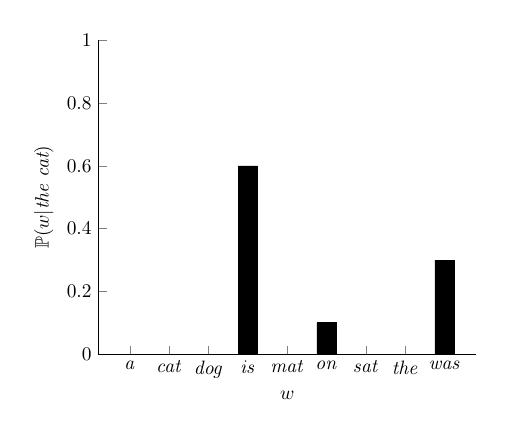
\begin{tikzpicture}[scale=0.7]
\begin{axis}[
	symbolic x coords={\tit{a}, \tit{cat}, \tit{dog}, \tit{is}, \tit{mat}, \tit{on}, \tit{sat}, \tit{the}, \tit{was}},
	xtick=data,
	xlabel={$w$},
	ylabel={$\mathbb{P}(w | \tit{the cat})$},
	ymin=0, ymax=1,
	axis x line*=bottom,
	axis y line*=left,
]

\addplot[ybar, fill=black]
coordinates {(\tit{a}, 0)(\tit{cat}, 0)(\tit{dog}, 0)(\tit{is}, 0.6)(\tit{mat}, 0)(\tit{on}, 0.1)(\tit{sat}, 0)(\tit{the}, 0)(\tit{was}, 0.3)};

\end{axis}
\end{tikzpicture}}}
~~\vcenter{\hbox{\scalebox{1}{$\xrightarrow{\tit{smooth}}$}}}~~
\vcenter{\hbox{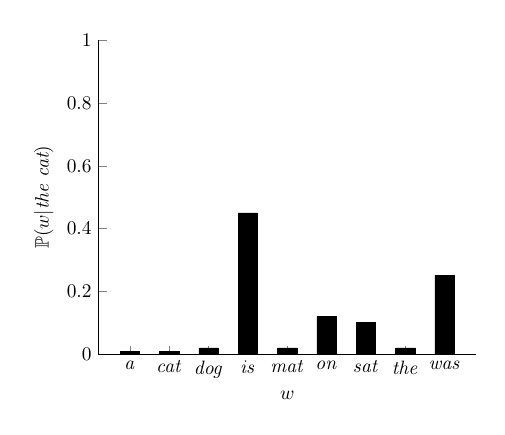
\begin{tikzpicture}[scale=0.7]
\begin{axis}[
	symbolic x coords={\tit{a}, \tit{cat}, \tit{dog}, \tit{is}, \tit{mat}, \tit{on}, \tit{sat}, \tit{the}, \tit{was}},
	xtick=data,
	xlabel={$w$},
	ylabel={$\mathbb{P}(w | \tit{the cat})$},
	ymin=0, ymax=1,
	axis x line*=bottom,
	axis y line*=left,
]

\addplot[ybar, fill=black]
coordinates {(\tit{a}, 0.01)(\tit{cat}, 0.01)(\tit{dog}, 0.02)(\tit{is}, 0.45)(\tit{mat}, 0.02)(\tit{on}, 0.12)(\tit{sat}, 0.1)(\tit{the}, 0.02)(\tit{was}, 0.25)};

\end{axis}
\end{tikzpicture}}}$
\caption{A toy example of smoothing, where the vocabulary is\\$V = \{$\tit{a}, \tit{cat}, \tit{dog}, \tit{is}, \tit{mat}, \tit{on}, \tit{sat}, \tit{the}, \tit{was}$\}$.}
\end{figure}

\subsection{Smoothing Techniques}

\subsubsection{Add-One Smoothing}

Add-one smoothing~\cite{add1_smoothing:johnson1932} simply involves adding 1 to each of the $n$-gram counts, and adding $|V|$ to the denominator ensure the probabilities sum to 1:
\begin{gather}
	\mathbb{P}(w_i | w_{i - n + 1}^{i - 1})_{\text{\scshape add-one}} = \frac{c(w_{i - n + 1}^{i}) + 1}{\sum_w c(w_{i - n + 1}^{i - 1}w) + |V|}
\end{gather}
One issue with add-one smoothing is that it gives an equal amount of probability to all $n$-grams, regardless of how likely they actually are. For example, if both \tit{`cat is'} and \tit{`cat pizza'} are unseen in the training data of a bigram model, then $\mathbb{P}(\tit{is}\ |\ \tit{cat})_{\text{\scshape add-one}} = \mathbb{P}(\tit{pizza}\ |\ \tit{cat})_{\text{\scshape add-one}}$. A simple way to reduce this problem is to employ \tit{backoff}, a technique whereby you recurse on the probability calculated by the $(n - 1)$-gram model. In this case, it is likely that $\mathbb{P}(\tit{is})_{\text{\scshape add-one}} > \mathbb{P}(\tit{pizza})_{\text{\scshape add-one}}$, which could be used to deduce that \tit{`cat is'} is more likely than \tit{`cat pizza'}.

\subsubsection{Absolute Discounting}

Absolute discounting employs backoff by interpolating higher and lower order $n$-gram models. It does this by subtracting a fixed discount $0 \leq D \leq 1$ from each non-zero count:
\begin{equation}
\begin{aligned}
	\mathbb{P}(w_i | w_{i - n + 1}^{i - 1})_{\text{\scshape ABS}} &= \frac{max\{c(w_{i - n + 1}^{i}) - D, 0\}}{\sum_w c(w_{i - n + 1}^{i - 1}w)} \\
	&+ \frac{D}{\sum_w c(w_{i - n + 1}^{i - 1}w)}N_{1+}(w_{i - n + 1}^{i - 1}\bullet)\mathbb{P}(w_i | w_{i - n + 2}^{i - 1})_{\text{\scshape ABS}}
\end{aligned}
\end{equation}
where
\begin{gather} \label{eq:n1plus}
	N_{1+}(w_{i - n + 1}^{i - 1}\bullet) = |\{ w\ |\ c(w_{i - n + 1}^{i - 1}w) \geq 1 \}|
\end{gather}
and the base case of recursion is given by $\mathbb{P}(w)_{\text{\scshape ABS}} = \mathbb{P}(w)_{\text{\scshape MLE}}$. $N_{1+}(w_{i - n + 1}^{i - 1}\bullet)$ is the number of unique words that follow the sequence $w_{i - n + 1}^{i - 1}$, which is the number of $n$-grams that $D$ is subtracted from. It is not difficult to show that the coefficient attached to the $\mathbb{P}(w_i | w_{i - n + 2}^{i - 1})_{\text{\scshape ABS}}$ term ensures that the probabilities sum to 1. \\

Ney, Essen and Kneser~\cite{absolute_discounting:ney1994} suggest setting $D$ to the value:
\begin{gather} \label{eq:discount}
	D = \frac{n_1}{n_1 + 2n_2}
\end{gather}
where $n_1$ and $n_2$ are the total number of $n$-grams with 1 and 2 counts respectively.

\subsubsection{Kneser-Ney Smoothing}

Kneser and Ney proposed an extension to absolute discounting which takes into account the number of unique words that precede a given $n$-gram~\cite{kneser_ney_smoothing:kneser1995}. As a motivating example, consider the bigrams \tit{`bottle cap'} and \tit{`bottle Francisco'}. If neither have been seen in the training data, and \tit{`Francisco'} occurs more frequently than \tit{`cap'}, then the absolute discounting model would backoff onto the unigram distribution and assign a higher probability to the \tit{`bottle Francisco'} bigram, despite the fact that \tit{`Francisco'} only ever follows \tit{`San'}. \\

From this example, it seems intuitive to assign more probability to those $n$-grams that follow a larger number of unique words. Kneser and Ney encapsulate this intuition by replacing some of the absolute counts $c(w_i^j)$ with the number of unique words that precede the word sequence $w_i^j$, $N_{1+}(\bullet w_i^j)$:
\begin{gather}
	N_{1+}(\bullet w_i^j) = |\{w\ |\ c(ww_i^j) \geq 1\}|
\end{gather}
Kneser-Ney smoothing\footnote{This is actually the interpolated version of Kneser-Ney smoothing, which differs slightly in form to the equation presented in the original paper.} is defined as follows:
\begin{align}
	\mathbb{P}(w_i | w_{i - n + 1}^{i - 1})_{\text{\scshape KN}} &= \frac{max\{\gamma(w_{i - n + 1}^{i}) - D, 0\}}{\sum_w \gamma(w_{i - n + 1}^{i - 1}w)} \\
	&+ \frac{D}{\sum_w \gamma(w_{i - n + 1}^{i - 1}w)}N_{1+}(w_{i - n + 1}^{i - 1}\bullet)\mathbb{P}(w_i | w_{i - n + 2}^{i - 1})_{\text{\scshape KN}}
\end{align}
where
\begin{gather} \label{eq:gamma}
	\gamma(w_{i - k + 1}^i) = \begin{cases}
		c(w_{i - k + 1}^i) &\text{for the outermost level of recursion (i.e. $k = n$)} \\
		N_{1+}(\bullet w_{i - k + 1}^i) &\text{otherwise}
	\end{cases}
\end{gather}
and the unigram probability is given as:
\begin{gather}
	\mathbb{P}(w_i)_{\text{\scshape KN}} = \frac{N_{1+}(\bullet w_i)}{\sum_w N_{1+}(\bullet w)}
\end{gather}

\subsubsection{Modified Kneser-Ney Smoothing}

Chen and Goodman noticed that the ideal average discount value, $D$, for $n$-grams with one or two counts is substantially different from the ideal average discount for $n$-grams with higher counts. Upon this discovery, they introduced a modified version of Kneser-Ney smoothing~\cite{modified_kneser_ney:chen1999}:
\begin{equation}
\begin{aligned}
	\mathbb{P}(w_i | w_{i - k + 1}^{i - 1})_{\text{\scshape MKN}} &= \frac{max\{\gamma(w_{i - k + 1}^{i}) - D(c(w_{i - k + 1}^{i}), 0\}}{\sum_w \gamma(w_{i - k + 1}^{i - 1}w)} \\
	&+ \lambda(w_{i - k + 1}^{i - 1})\mathbb{P}(w_i | w_{i - k + 2}^{i - 1})_{\text{\scshape MKN}}
\end{aligned}
\end{equation}
where $\gamma$ is defined in equation \ref{eq:gamma}, and $\lambda$ is defined as:
\begin{gather}
	\lambda(w_{i - k + 1}^{i - 1}) = \frac{D_1N_1(w_{i - k + 1}^{i - 1}\bullet) + D_2N_2(w_{i - k + 1}^{i - 1}\bullet) + D_{3+}N_{3+}(w_{i - k + 1}^{i - 1}\bullet)}{\sum_w \gamma(w_{i - k + 1}^{i - 1}w)}
\end{gather}
and
\begin{gather}
	D(c) = \begin{cases}
		0 &\text{if }c = 0 \\
		D_1 &\text{if }c = 1 \\
		D_2 &\text{if }c = 2 \\
		D_{3+} &\text{if }c \geq 3 \\
	\end{cases}
\end{gather}
where $N_1$, $N_2$ and $N_{3+}$ are defined analogously to $N_{1+}$ in equation~\ref{eq:n1plus}. Chen and Goodman suggest:
\begin{align}
	D_1 = 1 - 2D\frac{n_2}{n_1} && D_2 = 2 - 3D\frac{n_3}{n_2} && D_{3+} = 3 - 4D\frac{n_4}{n_3}
\end{align}
where $D$ is as defined in equation \ref{eq:discount}.

\subsubsection{Katz Smoothing}

Katz smoothing is a popular smoothing technique based on the Good-Turing estimate~\cite{good_turing:good1953}, which states that an $n$-gram that occurs $r$ times should be treated as occurring $r^*$ times, where:
\begin{gather}
	r^* = (r + 1)\frac{n_{r + 1}}{n_r}
\end{gather}
and $n_r$ is the number of $n$-grams that occur $r$ times. Converting this count into a probability simply involves normalising as follows:
\begin{gather} \label{eq:gt}
	\mathbb{P}(w_i | w_{i - n + 1}^{i - 1})_{\text{\scshape GT}} = \frac{c^*(w_{i - n + 1}^{i})}{\sum_{r = 0}^\infty n_r r^*}
\end{gather}
Katz smoothing~\cite{katz_smoothing:katz1987} is then defined as:
\begin{gather} \label{eq:katz}
	\mathbb{P}(w_i | w_{i - n + 1}^{i - 1})_{\text{\scshape KATZ}} = \begin{cases}
		\mathbb{P}(w_i | w_{i - n + 1}^{i - 1})_{\text{\scshape GT}} &\text{if }c(w_{i - n + 1}^i) > 0 \\
		\alpha(w_{i - n + 1}^{i - 1})\mathbb{P}(w_i | w_{i - n + 2}^{i - 1})_{\text{\scshape KATZ}} &\text{otherwise}
	\end{cases}
\end{gather}
where
\begin{gather}
	\alpha(w_{i - n + 1}^{i - 1}) = \frac{1 - \sum_{\{w_i\ |\ c(w_{i - n + 1}^i) > 0\}} \mathbb{P}(w_i | w_{i - n + 1}^{i - 1})_{\text{\scshape KATZ}}}{1 - \sum_{\{w_i\ |\ c(w_{i - n + 1}^i) > 0\}} \mathbb{P}(w_i | w_{i - n + 2}^{i - 1})_{\text{\scshape KATZ}}}
\end{gather}
In practice, the infinite sum in equation \ref{eq:gt} cannot be computed. To get around this issue, Katz takes $n$-grams with counts above some threshold $k$ as reliable and only applies the Good-Turing estimate to those with a count less than or equal to $k$. Katz suggests $k = 5$. This modification requires a slightly different equation to \ref{eq:katz} and is presented in Katz's original paper.

\section{Recurrent Neural Network Models}

In this section I give a brief introduction to neural networks, recurrent neural networks (RNNs) and how RNNs can be used in the context of language modelling.

\subsection{An Overview of Neural Networks}

The human brain is a furiously complicated organ, packed with a network of approximately 86 billion neurons\footnote{According to a study by Azevedo et al.~\cite{brain_size:azevedo2009}.} that propagate electrochemical signals across connections called synapses. (Artificial) neural networks were originally developed as a mathematical model of the brain~\cite{nn_calculus:mcculloch1943}, which despite being substantially oversimplified, now provide an effective tool for classification and regression in modern-day machine learning. \\

\begin{figure}[h]
\captionsetup{justification=centering}
\centering
\begin{subfigure}{0.5\linewidth}
	\centering
	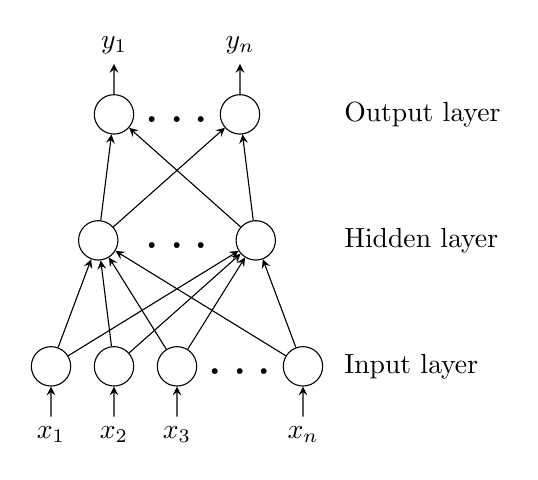
\begin{tikzpicture}[
		scale=0.8,
		every neuron/.style={circle, draw, minimum size=5mm},
		neuron missing/.style={draw=none, scale=2, text height=0.1cm, execute at begin node=\color{black}$\hdots$},
		>=stealth
	]

	\foreach \m/\l [count=\x] in {1, 2, 3, missing, 4}
		\node [every neuron/.try, neuron \m/.try] (input-\m) at (\x - 2.5, 0) {};

	\foreach \m [count=\x] in {1, missing, 2}
		\node [every neuron/.try, neuron \m/.try ] (hidden-\m) at (\x*1.25 - 2, 2) {};

	\foreach \m [count=\x] in {1, missing, 2}
		\node [every neuron/.try, neuron \m/.try ] (output-\m) at (\x - 1.5, 4) {};

	\foreach \l [count=\i] in {1, 2, 3, n}
		\draw [<-] (input-\i) -- ++(0, -0.8) node [below] {$x_\l$};

	\foreach \l [count=\i] in {1, n}
		\node [above] at (hidden-\i.north) {};

	\foreach \l [count=\i] in {1, n}
		\draw [->] (output-\i) -- ++(0, 0.8) node [above] {$y_\l$};

	\foreach \i in {1, ..., 4}
		\foreach \j in {1, ..., 2}
			\draw [->] (input-\i) -- (hidden-\j);

	\foreach \i in {1, ..., 2}
		\foreach \j in {1, ..., 2}
			\draw [->] (hidden-\i) -- (output-\j);

	\foreach \l [count=\y from 0] in {Input, Hidden, Output}
		\node [right] at (3, \y*2) {\l\ layer};
	\end{tikzpicture}
	\caption{An example multilayer perceptron.}
\end{subfigure}%
\begin{subfigure}{0.5\linewidth}
	\centering
	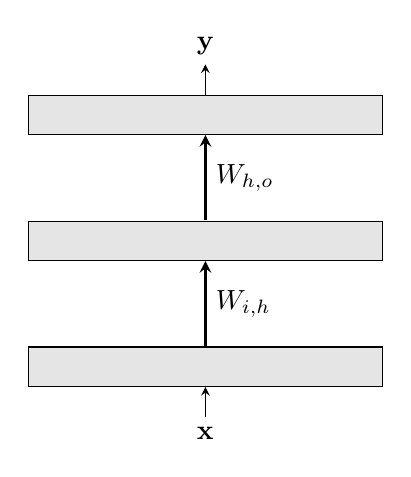
\begin{tikzpicture}[
		scale=0.8,
		>=stealth
	]

	\node[draw, rectangle, minimum width=45mm, minimum height=5mm, fill=black!10, ] (input) at (0, 0) {};
	\node[draw, rectangle, minimum width=45mm, minimum height=5mm, fill=black!10] (hidden) at (0, 2) {};
	\node[draw, rectangle, minimum width=45mm, minimum height=5mm, fill=black!10] (output) at (0, 4) {};
	\draw [<-] (input) -- ++(0, -0.8) node [below] {$\mathbf{x}$};
	\draw [->, line width=0.3mm] (input) to node [right] {$W_{i,h}$} (hidden);
	\draw [->, line width=0.3mm] (hidden) to node [right] {$W_{h,o}$} (output);
	\draw [->] (output) -- ++(0, 0.8) node [above] {$\mathbf{y}$};

	\end{tikzpicture}
	\caption{A simplified notation for (a).}
\end{subfigure}
\caption{Two alternative notations for the same network.}
\end{figure}

Neural networks consist of a series of nodes which are joined by directed and weighted connections. Inputs are supplied to some subset of the nodes and then propagated along the weighted connections until they reach the designated output nodes. In the context of the brain, the nodes represent neurons, the weighted connections represent synapses and the flow of information represents electrochemical signals. \\

An important distinction to be made is whether the neural network is cyclic or not. Acyclic neural networks are called feed-forward neural networks (FNNs), whereas cyclic neural networks are denoted recurrent neural networks (RNNs) which are covered in section \ref{rnns}. There are a variety of FNNs, but the most prominent is the multilayer perceptron (MLP)~\cite{backprop:rumelhart1985}.

\subsubsection{The Multilayer Perceptron}

The multilayer perceptron consists of layers of neurons, where each layer is fully connected to the next one. The first and last layers are the input and output layers, and any layers in between are called \tit{hidden layers}. The input neurons simply pass on the input values that they are given. Neurons in the subsequent layers, however, compute the following:

\begin{figure}[h]
\captionsetup{justification=centering}
\begin{center}
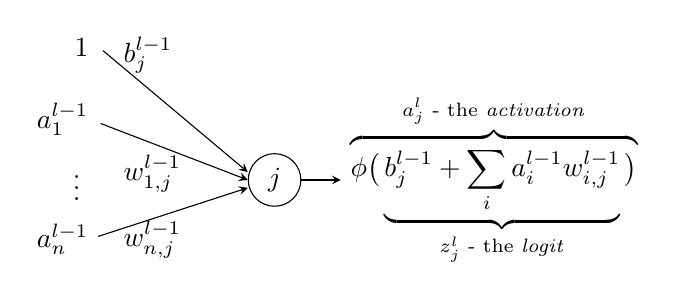
\begin{tikzpicture}[
	every neuron/.style={circle, draw, minimum size=5mm},
	neuron missing/.style={draw=none, scale=2, text height=0.1cm, execute at begin node=\color{black}$\hdots$},
	x=1.5cm,
	y=1.5cm,
	>=stealth
]

\node[every neuron/.try] (neuron) {$j$};
\node[left=10mm of neuron] (mid) {};
\node[above left=12mm and 20mm of neuron] (bias) {$1$};
\node[above left=2mm and 20mm of neuron] (inp1) {$a_1^{l-1}$};
\node[left=20mm of neuron] (var) {$\vdots$};
\node[below left=2mm and 20mm of neuron] (inpN) {$a_n^{l-1}$};

\draw[<-] (neuron.west |- mid) coordinate (aux)--++(159:20mm) node [below right=0mm and 2mm of inp1] {$w_{1,j}^{l-1}$};
\draw[<-] ([yshift=1mm]aux)--++(140:24mm) node [below right=-5mm and 2mm of bias] {$b_j^{l-1}$};
\draw[<-] ([yshift=-1mm]aux)--++(-162:20mm) node [right=2mm of inpN] {$w_{n,j}^{l-1}$};

\draw[->] (neuron.east) -- ++(0:5mm) node [right] {$\overbrace{\phi \big( \underbrace{b_j^{l - 1} + \sum_i a_i^{l - 1} w_{i,j}^{l-1}}_{z_j^l\text{ - the \tit{logit}}} \big)}^{a_j^l\text{ - the \tit{activation}}}$};

\end{tikzpicture}
\caption{The computation carried out by each neuron. The outputs or \tit{activations} of the neurons from the previous layer, $(l - 1)$, are denoted $a_i^{l-1}$, the weights on the input connections are $w_{i,j}^{l-1}$, the \tit{activation function} is $\phi$ and $b_j^{l - 1}$ is the bias variable.}
\label{fig:neuron}
\end{center}
\end{figure}

The constant-valued input 1 is known as a \tit{bias} input, which is weighted by a bias variable $b_j^{l - 1}$. Its purpose is to allow the neuron to shift the output of the activation function left and right by adjusting the value of $b_j^{l - 1}$. Bias inputs are usually attached to every non-input neuron in the network. \\

Activation functions were originally created to mimic the firing activity of neurons. It is important that they are chosen to be non-linear. Any combination of linear operators is linear, which means that any linear MLP with multiple hidden layers is equivalent to an MLP with a single hidden layer. Non-linear neural networks, on the other hand, are more powerful, and can gain considerable performance by adding successive hidden layers to re-represent the input data at higher levels of abstraction~\cite{dbn:hinton2006}~\cite{scaling:bengio2007}. In fact, is has been shown that a non-linear MLP with a single hidden layer containing a sufficient number of neurons can approximate any continuous function on a compact input domain to arbitrary precision~\cite{universal_approximators:hornik1989}. \\

Frequently used activation functions include the sigmoid and the hyperbolic tangent functions. Another important property of these functions is that they are differentiable, which allows for the network to be trained using \tit{gradient descent}, which is discussed below. \\

\begin{figure}[h]
\captionsetup{justification=centering}
\centering
\begin{subfigure}{0.5\linewidth}
	\centering
	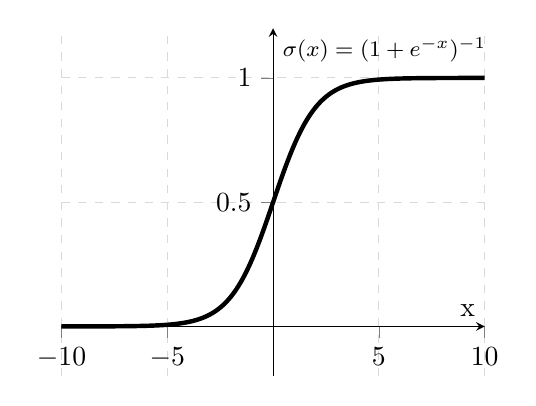
\begin{tikzpicture}
	\begin{axis}[
		height=6cm,
		legend pos=north west,
		axis x line=middle,
		axis y line=middle,
		grid = major,
		grid style={dashed, gray!30},
		xmin=-10, xmax= 10,
		ymin= -0.2, ymax= 1.2,
		xlabel=x,
		ylabel={\footnotesize $\sigma(x) = (1 + e^{-x})^{-1}$},
		tick align=outside,
		enlargelimits=false]
	\addplot[domain=-10:10, black, ultra thick,samples=500] {1/(1+exp(-x))};
	\end{axis}
	\end{tikzpicture}
	\caption{The sigmoid function, $\sigma$.}
\end{subfigure}%
\begin{subfigure}{0.5\linewidth}
	\centering
	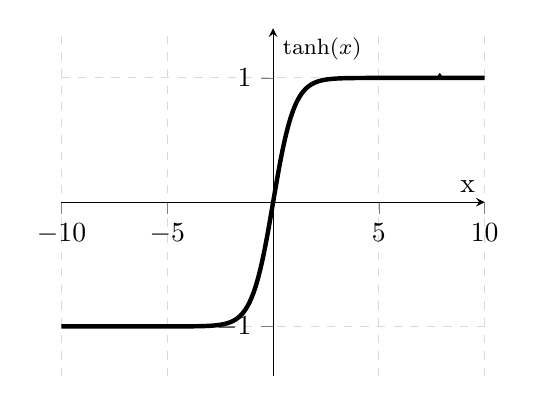
\begin{tikzpicture}
	\begin{axis}[
		height=6cm,
		legend pos=north west,
		axis x line=middle,
		axis y line=middle,
		grid = major,
		grid style={dashed, gray!30},
		xmin=-10, xmax= 10,
		ymin= -1.4, ymax= 1.4,
		xlabel=x,
		ylabel={\footnotesize $\tanh (x)$},
		tick align=outside,
		enlargelimits=false]
	\addplot[domain=-10:10, black, ultra thick,samples=500] {(exp(x) - exp(-x))/(exp(x) + exp(-x))};
	\end{axis}
	\end{tikzpicture}
	\caption{The hyperbolic tangent function, $\tanh$.}
\end{subfigure}
\caption{Two popular activation functions.}
\end{figure}

\subsubsection{Backpropagation and Gradient Descent}

FNNs compute a function, $f$, parameterised by the weights $\mathbf{w}$ of the network, mapping an input vector $\mathbf{x} = (x_1, ..., x_n)^T$ to an output vector $\mathbf{y} = (y_1, ..., y_m)^T$. 
\begin{gather*}
	\mathbf{y} = f_\mathbf{w}(\mathbf{x})
\end{gather*}
The entire point of training a neural network is to get it to learn a particular mapping from input vectors to output vectors. What these vectors represent depends on the problem at hand. For example, in the context of classifying pictures of animals, the input vector might represent the pixel values of an image and the output vector might represent a probability distribution over the set of animals in the classification task. \\

In order to train a neural network, you supply it with a training set, which is just a list of input-target pairs:
\begin{gather*}
	\mathbf{s} = ((\mathbf{x}_1, \mathbf{t}_1), ..., (\mathbf{x}_N, \mathbf{t}_N))
\end{gather*}
where $\mathbf{t}_k$ is the vector that the network should output given the example input $\mathbf{x}_k$. A differentiable loss function, $\mathcal{L}(\mathbf{y}, \mathbf{t})$, is also defined, which essentially says how badly the network output $\mathbf{y}$ matches the target output $\mathbf{t}$. Then, a measure of how much error the network produces over the whole training set can be defined as follows:
\begin{gather}
	\mathcal{L}_{\text{\scshape total}} = \sum_{k = 1}^N \mathcal{L}(f_{\mathbf{w}}(\mathbf{x}_k), \mathbf{t}_k)
\end{gather}
The end product of the \tit{backpropagation} algorithm is the partial derivative:
\begin{gather*}
	\frac{\partial}{\partial w_{i,j}^l} \big( \mathcal{L}_{\text{\scshape total}} \big)
\end{gather*}
for every weight $w_{i,j}^l$ in the neural network. It is a two stage algorithm that works as follows:
\begin{enumerate}
\item
	Calculate, $f_{\mathbf{w}}(\mathbf{x}_k)$ for each input example $\mathbf{x}_k$, and use those values to derive $\mathcal{L}_{\text{\scshape total}}$.
\item
	Given $\mathcal{L}_{\text{\scshape total}}$, calculate $\frac{\partial}{\partial w_{i,j}^l} \big( \mathcal{L}_{\text{\scshape total}} \big)$ for each weight in each layer of the network by applying the chain rule backwards from the output layer to the input layer.
\end{enumerate}

$\frac{\partial}{\partial w_{i,j}^l} \big( \mathcal{L}_{\text{\scshape total}} \big)$ is calculated as follows:
\begin{gather} \label{eq:bp_weight_grad}
	\frac{\partial}{\partial w_{i,j}^l} \big( \mathcal{L}_{\text{\scshape total}} \big) = \sum_{k = 1}^N \underbrace{\frac{\partial \mathcal{L}}{\partial f_{\mathbf{w}}(\mathbf{x}_k)}  \frac{\partial f_{\mathbf{w}}(\mathbf{x}_k)}{\partial z_j^{l + 1}}}_{\delta_j^{l+1}}  \frac{\partial z_j^{l + 1}}{\partial w_{i,j}^l} = \delta_j^{l+1} a_i^l
\end{gather}
The delta term $\delta_j^{l+1}=\frac{\partial \mathcal{L}}{\partial z_j^{l + 1}}$ varies in form for each layer. For the output layer, it has the following form:
\begin{gather} \label{eq:delta_output}
	\delta_j^L = \frac{\partial \mathcal{L}}{\partial f_{\mathbf{w}}(\mathbf{x}_k)} \phi'(z_j^L)
\end{gather}
For the preceding layers, $\delta_j^l$ can be defined recursively in terms of the delta values for the neurons in subsequent layers in the network. This is defined below, and a detailed justification of it is given in appendix \ref{appendix:bp_recurrence}:
\begin{gather} \label{eq:delta_hidden}
	\delta_i^l = \phi'(z_i^l) \sum_j \delta_j^{l+1} w_{i,j}^l
\end{gather}

\tit{Gradient descent} is an optimisation technique that uses the derivatives produced by the backpropagation algorithm to adjust the weights such that the loss is minimised over the training set. It does this by changing each weight value in the direction of the negative gradient of the loss, which can be visualised as moving downhill on the error surface plotted with respect to the weights in the network:
\begin{gather}
	w_{i,j}^l \leftarrow w_{i,j}^l - \eta \frac{\partial}{\partial w_{i,j}^l} \big( \mathcal{L}_{\text{\scshape total}} \big)
\end{gather}
$\eta > 0$ is known as the \tit{learning rate}, which determines how large the steps are in the negative direction of the gradient. Ways for setting $\eta$, and other useful techniques when training neural networks in practice are described in chapter \ref{implementation}.

\subsection{Recurrent Neural Networks} \label{rnns}

In the context of language modelling, the input is a sequence of words and the output is a sequence of probability distributions over the possible next words at each point. Ideally, the word with the highest probability at each step should be the next word in the input sequence. For example, given (\tit{`the', `cat', `sat', ...}) as input, the network should produce something along the lines of (~%
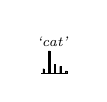
\begin{tikzpicture}[scale=0.05]
\begin{axis}[
	clip=false,
	hide y axis,
	axis x line*=bottom,
	ymin=0, ymax=5,
	xticklabels={,,,,},
]
\addplot[ybar, fill=black]
coordinates {(1, 1)(2, 5)(3, 2)(4, 1.5)(5, 0.5)};
\end{axis}
\node at (3, 8) {\tiny \tit{`cat'}};
\end{tikzpicture}, %
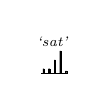
\begin{tikzpicture}[scale=0.05]
\begin{axis}[
	clip=false,
	hide y axis,
	axis x line*=bottom,
	ymin=0, ymax=5,
	xticklabels={,,,,},
]
\addplot[ybar, fill=black]
coordinates {(1, 1)(2, 1)(3, 3)(4, 5)(5, 0.5)};
\end{axis}
\node at (3, 8) {\tiny \tit{`sat'}};
\end{tikzpicture}, %
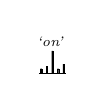
\begin{tikzpicture}[scale=0.05]
\begin{axis}[
	clip=false,
	hide y axis,
	axis x line*=bottom,
	ymin=0, ymax=5,
	xticklabels={,,,,},
]
\addplot[ybar, fill=black]
coordinates {(1, 1)(2, 1.5)(3, 5)(4, 1)(5, 2)};
\end{axis}
\node at (3, 8) {\tiny \tit{`on'}};
\end{tikzpicture}, %
... ) as output. The problem with FNNs is that these sequences may have varying length, yet FNNs have fixed input and output vector sizes. Recurrent neural networks (RNNs) naturally lend themselves to tackling this issue. \\

\begin{figure}[h]
\captionsetup{justification=centering}
\centering
\begin{subfigure}{0.3\linewidth}
	\centering
	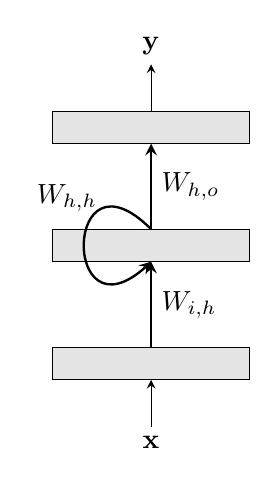
\begin{tikzpicture}[>=stealth]
		\node[draw, rectangle, minimum width=25mm, minimum height=4mm, fill=black!10, ] (input) at (0, 0) {};
		\node[draw, rectangle, minimum width=25mm, minimum height=4mm, fill=black!10] (hidden) at (0, 1.5) {};
		\node[draw, rectangle, minimum width=25mm, minimum height=4mm, fill=black!10] (output) at (0, 3) {};
		\draw [<-] (input) -- ++(0, -0.8) node [below] {$\mathbf{x}$};
		\draw [->, line width=0.3mm] (input) to node [right] {$W_{i,h}$} (hidden);
		\draw [->, line width=0.3mm, out=135, in=225, looseness=10] (hidden.north) to node [above left=3mm and -3mm of hidden] {$W_{h,h}$} (hidden.south);
		\draw [->, line width=0.3mm] (hidden) to node [right] {$W_{h,o}$} (output);
		\draw [->] (output) -- ++(0, 0.8) node [above] {$\mathbf{y}$};
	\end{tikzpicture}
	\caption{An RNN.}
	\label{fig:rnn}
\end{subfigure}%
\begin{subfigure}{0.7\linewidth}
	\centering
	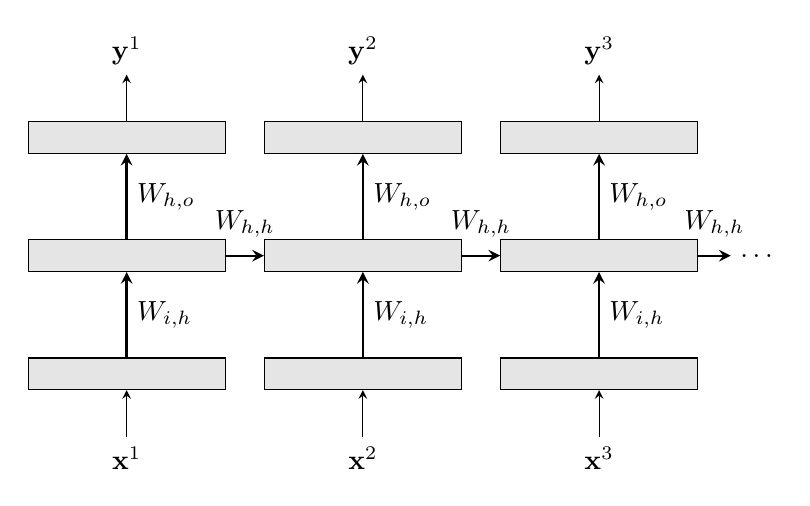
\begin{tikzpicture}[>=stealth]
		\node[draw, rectangle, minimum width=25mm, minimum height=4mm, fill=black!10, ] (input1) at (0, 0) {};
		\node[draw, rectangle, minimum width=25mm, minimum height=4mm, fill=black!10] (hidden1) at (0, 1.5) {};
		\node[draw, rectangle, minimum width=25mm, minimum height=4mm, fill=black!10] (output1) at (0, 3) {};
		\draw [<-] (input1) -- ++(0, -0.8) node [below] {$\mathbf{x}^1$};
		\draw [->, line width=0.3mm] (input1) to node [right] {$W_{i,h}$} (hidden1);
		\draw [->, line width=0.3mm] (hidden1) to node [right] {$W_{h,o}$} (output1);
		\draw [->] (output1) -- ++(0, 0.8) node [above] {$\mathbf{y}^1$};

		\node[draw, rectangle, minimum width=25mm, minimum height=4mm, fill=black!10, ] (input2) at (3, 0) {};
		\node[draw, rectangle, minimum width=25mm, minimum height=4mm, fill=black!10] (hidden2) at (3, 1.5) {};
		\node[draw, rectangle, minimum width=25mm, minimum height=4mm, fill=black!10] (output2) at (3, 3) {};
		\draw [<-] (input2) -- ++(0, -0.8) node [below] {$\mathbf{x}^2$};
		\draw [->, line width=0.3mm] (input2) to node [right] {$W_{i,h}$} (hidden2);
		\draw [->, line width=0.3mm] (hidden2) to node [right] {$W_{h,o}$} (output2);
		\draw [->] (output2) -- ++(0, 0.8) node [above] {$\mathbf{y}^2$};

		\node[draw, rectangle, minimum width=25mm, minimum height=4mm, fill=black!10, ] (input3) at (6, 0) {};
		\node[draw, rectangle, minimum width=25mm, minimum height=4mm, fill=black!10] (hidden3) at (6, 1.5) {};
		\node[draw, rectangle, minimum width=25mm, minimum height=4mm, fill=black!10] (output3) at (6, 3) {};
		\draw [<-] (input3) -- ++(0, -0.8) node [below] {$\mathbf{x}^3$};
		\draw [->, line width=0.3mm] (input3) to node [right] {$W_{i,h}$} (hidden3);
		\draw [->, line width=0.3mm] (hidden3) to node [right] {$W_{h,o}$} (output3);
		\draw [->] (output3) -- ++(0, 0.8) node [above] {$\mathbf{y}^3$};

		\node (cont) at (8, 1.5) {$\hdots$};

		\draw [->, line width=0.3mm] (hidden1.east) to node [above=1mm of hidden1] {$W_{h,h}$} (hidden2.west);
		\draw [->, line width=0.3mm] (hidden2.east) to node [above=1mm of hidden2] {$W_{h,h}$} (hidden3.west);
		\draw [->, line width=0.3mm] (hidden3.east) to node [above=1mm of hidden3] {$W_{h,h}$} (cont.west);
	\end{tikzpicture}
	\caption{An \tit{unrolled} RNN.}
	\label{fig:rnn_unrolled}
\end{subfigure}
\caption{Two different representations of the same RNN.}
\end{figure}

A recurrent neural network can be constructed from an FNN by adding connections from each neuron in a hidden layer back to every neuron in that layer, including itself. A nice property about RNNs is that they can be unrolled to an arbitrary number of steps without the need for any additional parameters, because the same weight matrices are reused at each step. For this reason, RNNs are well suited for operating over sequences of input data, which is of course ideal in the context of language modelling. The problem of representing textual words as numerical input vectors for an RNN is addressed in section \ref{word_embeddings}. \\

In most applications, the sequences of input vectors are typically ordered by time, so I use the notation $\mathbf{x}^t$ and $\mathbf{y}^t$ to denote the input and output vectors at time step $t$.

\subsubsection{Backpropagation Through Time (BPTT)}

Training an RNN is not so much different to training an FNN: the only difference is that gradients must also be calculated across time steps. As shown figure \ref{fig:rnn_unrolled}, each weight is reused at every time step, so the weight derivative is now summed across the time steps:
\begin{gather}
	\frac{\partial}{\partial w_{i,j}^l} \big( \mathcal{L}_{\text{\scshape total}} \big) = \sum_t \delta_j^{l+1,t} a_i^{l,t}
\end{gather}
The delta term for the output layer is defined analogously to equation \ref{eq:delta_output}:
\begin{gather} \label{eq:delta_output_rnn}
	\delta_j^{L,t} = \frac{\partial \mathcal{L}}{\partial f_{\mathbf{w}}(\mathbf{x}_k^t)} \phi'(z_j^{L,t})
\end{gather}
The delta term for the preceding layers can be shown to have the form below. This is justified in more detail in appendix \ref{appendix:bp_recurrence}:
\begin{gather} \label{eq:delta_hidden_rnn}
	\delta_i^{l,t} = \phi'(z_i^{l,t}) \big( \sum_j \delta_j^{l+1,t} w_{i,j}^l + \sum_j \delta_j^{l,t+1} v_{i,j}^l \big)
\end{gather}
where $v_{i,j}^l$ denotes the weight on the recurrent connection from neuron $i$ in layer $l$ back to neuron $j$ in the same layer.

\subsubsection{RNN Architectures}
So far, the equations presented have assumed a \tit{vanilla RNN}. That is, the $j^{th}$ neuron, or \tit{cell}, in layer $l$ at time step $t$ simply computes:
\begin{gather}
	a_j^{l, t} = \phi \big( \sum_i a_i^{l - 1, t} w_{i,j}^{l-1} + \sum_i a_i^{l, t - 1} v_{i,j}^l + b^{l - 1}_j \big)
\end{gather}
This computation can be written for an entire layer of hidden neurons, $\mathbf{a}^{l, t} = (a_1^{l, t}, a_2^{l, t}, ..., a_H^{l, t})$, using matrix notation as follows:
\begin{gather} \label{eq:vanilla_rnn}
	\mathbf{a}^{l, t} = \phi \big( \mathbf{W}^{l - 1} \mathbf{a}^{l - 1, t} + \mathbf{V}^l \mathbf{a}^{l, t - 1} + \mathbf{b}^{l - 1} \big)
\end{gather}
Various improvements to this architecture have been proposed, which capture longer-term information across the inputs. In this project, I have implemented the two most prominent alternatives, which are Long Short-Term Memory (LSTM)~\cite{lstm:hochreiter1997} and the Gated Recurrent Unit (GRU)~\cite{gru:cho2014}. These are outlined in figure~\ref{fig:rnn_architectures} and discussed in much more detail in section~\ref{architectures}. \\

\begin{figure}[h]
\captionsetup{justification=centering}
\centering
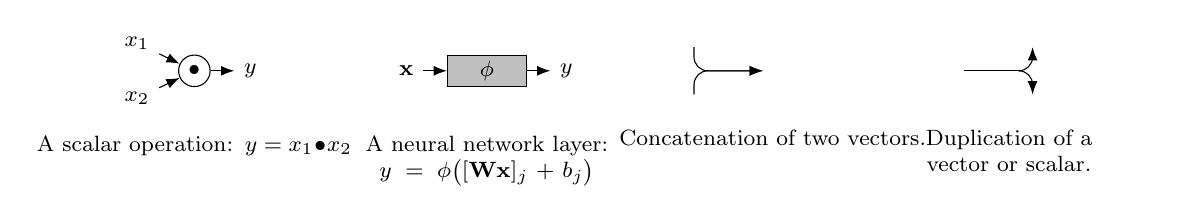
\begin{tikzpicture}[
	scalar/.style={circle, draw, inner sep=0pt, minimum width=4mm, font=\footnotesize},
	nnlayer/.style={rectangle, draw, inner sep=0pt, fill=gray!50, minimum width=10mm, minimum height=4mm, font=\footnotesize},
	textb/.style={minimum width=6mm, minimum height=4mm, text width=40mm, align=center, font=\footnotesize},
	>=LaTeX
]

\node[nnlayer] (nnlayer) {$\phi$};
\node[left=3mm of nnlayer] (nnlayer_input) {\footnotesize $\mathbf{x}$};
\node[right=3mm of nnlayer] (nnlayer_output) {\footnotesize $y$};
\node[textb, below=5mm of nnlayer] (nnlayertext) {A neural network layer: $y = \phi \big([\mathbf{W} \mathbf{x}]_j + b_j \big)$};

\node[scalar, left=30mm of nnlayer] (scalar) {$\bullet$};
\node[above left=0mm and 3mm of scalar] (scalar_input1) {\footnotesize $x_1$};
\node[below left=0mm and 3mm of scalar] (scalar_input2) {\footnotesize $x_2$};
\node[right=3mm of scalar] (scalar_output) {\footnotesize $y$};
\node[textb, below=5mm of scalar] (scalartext) {A scalar operation: $y = x_1 \bullet x_2$};

\node[right=30mm of nnlayer] (concat) {};
\node[textb, below=5mm of concat] (concattext) {Concatenation of two vectors.};

\node[right=60mm of nnlayer] (copy) {};
\node[textb, below=5mm of copy] (copytext) {Duplication of a vector or scalar.};

\draw[->] (nnlayer_input) -- (nnlayer);
\draw[->] (nnlayer) -- (nnlayer_output);

\draw[->] (scalar_input1) -- (scalar);
\draw[->] (scalar_input2) -- (scalar);
\draw[->] (scalar) -- (scalar_output);

\draw[<-, rounded corners=5pt] (concat) -| ++(-10mm,3mm);
\draw[<-, rounded corners=5pt] (concat) -| ++(-10mm,-3mm);

\draw[rounded corners=5pt] (copy.east) -- ++(-7mm,0mm);
\draw[->, rounded corners=5pt] (copy) -| ++(3mm,3mm);
\draw[->, rounded corners=5pt] (copy) -| ++(3mm,-3mm);

\end{tikzpicture}
\caption{A notation for drawing RNN architectures.}
\label{fig:rnn_notation}
\end{figure}

\begin{figure}[h]
\captionsetup{justification=centering}
\centering
\begin{subfigure}{0.33\linewidth}
	\centering
	\resizebox{4cm}{3cm}{%
	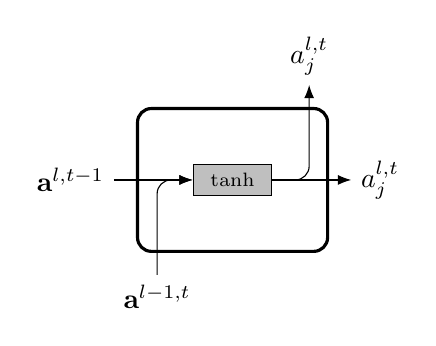
\begin{tikzpicture}[
		scalar/.style={circle, draw, inner sep=0pt, minimum width=4mm},
		tanlayer/.style={rectangle, draw, inner sep=0pt, fill=gray!50, minimum width=10mm, minimum height=4mm},
		siglayer/.style={rectangle, draw, inner sep=0pt, fill=gray!50, minimum width=6mm, minimum height=4mm},
		textb/.style={minimum width=6mm, minimum height=4mm},
		ct/.style={circle, draw, inner sep=5pt, ultra thick, minimum width=10mm},
		ft/.style={circle, draw, minimum width=8mm, inner sep=1pt},
		filter/.style={circle, draw, minimum width=7mm, inner sep=1pt, path picture={\draw[thick, rounded corners] (path picture bounding box.center)--++(65:2mm)--++(0:1mm);
		\draw[thick, rounded corners] (path picture bounding box.center)--++(245:2mm)--++(180:1mm);}},
		mylabel/.style={font=\scriptsize\sffamily},
		>=LaTeX
	]
	
	\node[tanlayer] (tanh) {\scriptsize $\tanh$};
	\node[textb, anchor=east, left=10mm of tanh] (hin) {$\mathbf{a}^{l, t - 1}$};
	\node[textb, anchor=west, right=10mm of tanh] (hout) {$a_j^{l, t}$};
	\node[textb, anchor=north, below left=10mm and -1mm of tanh] (x) {$\mathbf{a}^{l - 1, t}$};
	\node[textb, anchor=south, above right=10mm and 1mm of tanh] (hout2) {$a_j^{l, t}$};
	\node[fit=(tanh), draw, inner xsep=7mm, inner ysep=7mm, rounded corners=5pt, line width=0.4mm] (fit) {};

	\foreach \i/\j in {hin/tanh.west, tanh.east/hout}
		\draw[->, rounded corners=5pt] (\i) -- (\j);

	\draw [->, rounded corners=5pt] (x.north) |- (tanh.west);

	\draw [->, rounded corners=5pt] (tanh.east) -| (hout2);

	\end{tikzpicture}}
	\caption{A vanilla RNN cell.}
\end{subfigure}%
\begin{subfigure}{0.33\linewidth}
	\centering
	\resizebox{4.8cm}{3cm}{%
	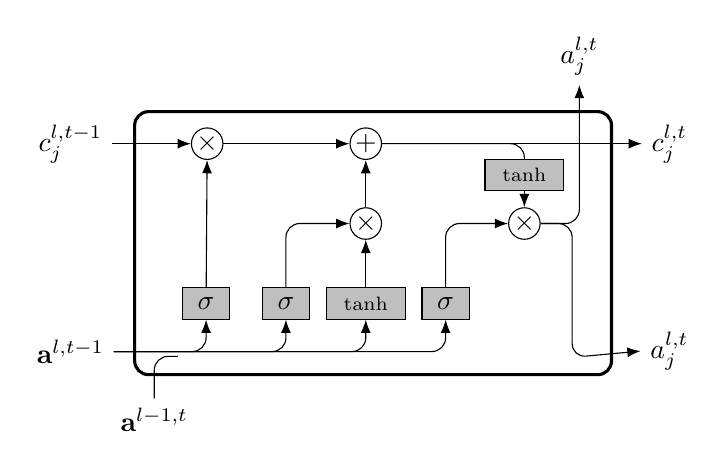
\begin{tikzpicture}[
		scalar/.style={circle, draw, inner sep=0pt, minimum width=4mm},
		tanlayer/.style={rectangle, draw, inner sep=0pt, fill=gray!50, minimum width=10mm, minimum height=4mm},
		siglayer/.style={rectangle, draw, inner sep=0pt, fill=gray!50, minimum width=6mm, minimum height=4mm},
		textb/.style={minimum width=6mm, minimum height=4mm},
		ct/.style={circle, draw, inner sep=5pt, ultra thick, minimum width=10mm},
		ft/.style={circle, draw, minimum width=8mm, inner sep=1pt},
		filter/.style={circle, draw, minimum width=7mm, inner sep=1pt, path picture={\draw[thick, rounded corners] (path picture bounding box.center)--++(65:2mm)--++(0:1mm);
		\draw[thick, rounded corners] (path picture bounding box.center)--++(245:2mm)--++(180:1mm);}},
		mylabel/.style={font=\scriptsize\sffamily},
		>=LaTeX
	]
	
	\node[scalar] (plus) {$+$};
	\node[scalar, left=16mm of plus] (ftimes) {$\times$};
	\node[scalar, below=6mm of plus] (itimes) {$\times$};
	\node[scalar, right=16mm of itimes] (otimes) {$\times$};
	\node[tanlayer, above=2mm of otimes] (otanh) {\scriptsize $\tanh$};
	\node[tanlayer, below=6mm of itimes] (stanh) {\scriptsize $\tanh$};
	\node[siglayer, left=2mm of stanh] (isig) {$\sigma$};
	\node[siglayer, left=4mm of isig] (fsig) {$\sigma$};
	\node[siglayer, right=2mm of stanh] (osig) {$\sigma$};
	\node[textb, anchor=east, left=10mm of ftimes] (Cin) {$c_j^{l, t - 1}$};
	\node[textb, anchor=east, below=20mm of Cin] (hin) {$\mathbf{a}^{l, t - 1}$};
	\node[textb, anchor=west, right=33mm of plus] (Cout) {$c_j^{l, t}$};
	\node[textb, anchor=west, below=19mm of Cout] (hout) {$a_j^{l, t}$};
	\node[textb, anchor=north, below left=10mm and -2mm of fsig] (x) {$\mathbf{a}^{l - 1, t}$};
	\node[textb, anchor=south, above right=6mm and 22mm of plus] (hout2) {$a_j^{l, t}$};
	\node[below=2.5mm of stanh] (invisible) {};
	\node[fit=(ftimes) (otanh) (osig) (fsig) (invisible), draw, inner xsep=6mm, inner ysep=2mm, rounded corners=5pt, line width=0.4mm] (fit) {};

	\foreach \i/\j in {otimes/hout2, hin/fsig, hin/isig, hin/stanh, hin/osig}
		\draw[->, rounded corners=5pt] (\i) -| (\j);

	\draw[-, rounded corners=5pt] (plus) -| (otanh);

	\foreach \i/\j in {isig/itimes, osig/otimes}
		\draw[->, rounded corners=5pt] (\i) |- (\j);

	\draw[->, rounded corners=5pt] (otimes.east) -| ++(4mm,-17mm) -- (hout.west);

	\foreach \i/\j in {Cin/ftimes, ftimes/plus, plus/Cout, fsig/ftimes, itimes/plus, stanh/itimes, otanh/otimes}
		\draw[->] (\i) -- (\j);

	\draw[-, rounded corners=5pt] (x.north) |- ++(3mm, 5.34mm);

	\end{tikzpicture}}
	\caption{An LSTM cell.}
\end{subfigure}%
\begin{subfigure}{0.33\linewidth}
	\centering
	\resizebox{4.8cm}{3cm}{%
	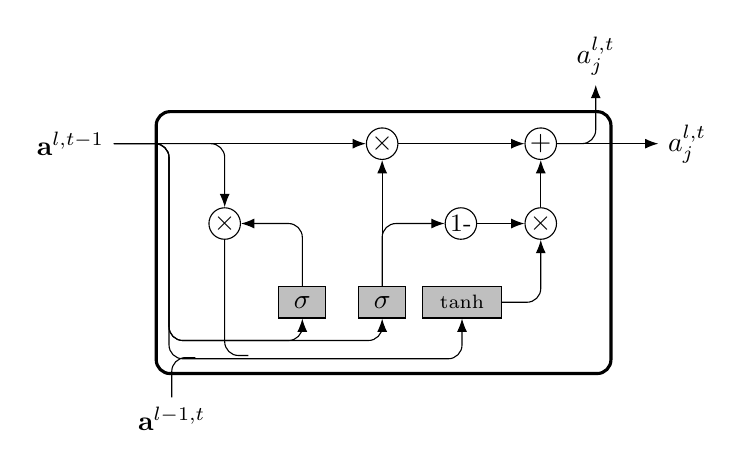
\begin{tikzpicture}[
		scalar/.style={circle, draw, inner sep=0pt, minimum width=4mm},
		tanlayer/.style={rectangle, draw, inner sep=0pt, fill=gray!50, minimum width=10mm, minimum height=4mm},
		siglayer/.style={rectangle, draw, inner sep=0pt, fill=gray!50, minimum width=6mm, minimum height=4mm},
		textb/.style={minimum width=6mm, minimum height=4mm},
		ct/.style={circle, draw, inner sep=5pt, ultra thick, minimum width=10mm},
		ft/.style={circle, draw, minimum width=8mm, inner sep=1pt},
		filter/.style={circle, draw, minimum width=7mm, inner sep=1pt, path picture={\draw[thick, rounded corners] (path picture bounding box.center)--++(65:2mm)--++(0:1mm);
		\draw[thick, rounded corners] (path picture bounding box.center)--++(245:2mm)--++(180:1mm);}},
		mylabel/.style={font=\scriptsize\sffamily},
		>=LaTeX
	]
	
	\node[scalar] (times) {$\times$};
	\node[scalar, right=16mm of times] (plus) {$+$};
	\node[scalar, below=6mm of plus] (times2) {$\times$};
	\node[scalar, left=6mm of times2] (minus1) {\small 1-};
	\node[scalar, left=36mm of times2] (times3) {$\times$};
	\node[siglayer, below=16mm of times] (sig2) {$\sigma$};
	\node[siglayer, left=4mm of sig2] (sig1) {$\sigma$};
	\node[tanlayer, right=2mm of sig2] (tanh) {\scriptsize $\tanh$};
	\node[textb, anchor=east, left=32mm of times] (hin) {$\mathbf{a}^{l, t - 1}$};
	\node[textb, anchor=west, right=33mm of times] (hout) {$a_j^{l, t}$};
	\node[textb, anchor=north, below left=10mm and 8mm of sig1] (x) {$\mathbf{a}^{l - 1, t}$};
	\node[textb, anchor=south, above right=6mm and 22mm of times] (hout2) {$a_j^{l, t}$};
	\node[below right=2.5mm and 17.5mm of sig2] (invisible) {};
	\node[left=7mm of sig1] (invisible2) {};
	\node[fit=(plus) (tanh) (invisible) (invisible2), draw, inner xsep=6mm, inner ysep=2mm, rounded corners=5pt, line width=0.4mm] (fit) {};

	\foreach \i/\j in {hin/times3, plus/hout2, tanh/times2}
		\draw[->, rounded corners=5pt] (\i) -| (\j);

	\foreach \i/\j in {sig1/times3, sig2/minus1}
		\draw[->, rounded corners=5pt] (\i) |- (\j);

	\foreach \i/\j in {hin/times, times/plus, plus/hout, times2/plus, minus1/times2, sig2/times}
		\draw[->] (\i) -- (\j);

	\foreach \i/\j in {hin.east/sig1.south, hin.east/sig2.south}
		\draw[->, rounded corners=5pt] (\i) -| ++(7mm,-25mm) -| (\j);
		
	\draw[->, rounded corners=5pt] (hin.east) -| ++(7mm,-27.32mm) -| (tanh.south);

	\draw[-, rounded corners=5pt] (times3.south) |- ++(3mm, -14.69mm);

	\draw[-, rounded corners=5pt] (x.north) |- ++(3mm, 5.045mm);

	\end{tikzpicture}}
	\caption{A GRU cell.}
\end{subfigure}
\caption{Various architectures of RNN neurons, using the notation from figure~\ref{fig:rnn_notation}. Each diagram represents the computation of the $j^{th}$ neuron or cell in layer $l$.}
\label{fig:rnn_architectures}
\end{figure}

\subsection{Word Embeddings} \label{word_embeddings}

In order for an RNN to take a sequence of words as input, each word must first be mapped to a vector representation, known as a \tit{word embedding}. Each word embedding represents a point in a high-dimensional space, and ideally, similar words will be assigned points which are closer together. In this dissertation, I get the RNN to learn good word embeddings through the application of backpropagation and gradient descent to the vector elements.

\section{Software Engineering}

This section details the project requirements and early design decisions that were made.

\subsection{Requirements}

The success requirements set out in the project proposal were:

\begin{center}
\begin{tabular}{L{1cm} L{14cm}}
	\hline
	\tbf{R1} & Language models (LMs) using the following techniques are implemented:
	\begin{itemize}[nosep]
	\item
		$n$-gram LMs with various smoothing techniques.
	\item
		A vanilla RNN-based LM.
	\item
		An LSTM-based LM.
	\end{itemize}\\[-\normalbaselineskip] \hline
	\tbf{R2} & Comprehensible and reliable comparisons between the various LM implementations and their combinations are made regarding their accuracy, speed and resource consumption during both training and inference. \\ \hline
	\tbf{R3} & A simple console application is developed to demonstrate the capability of the aforementioned language models in the context of next-word prediction. \\ \hline
\end{tabular}
\end{center}

The project proposal also suggested two possible extensions:
\begin{center}
\begin{tabular}{L{1cm} L{14cm}}
	\hline
	\tbf{E1} & Explore possible extensions to existing language models to improve their performance on error-prone text. \\ \hline
	\tbf{E2} & Build a mobile keyboard that exhibits the functionality of the language models. \\ \hline
\end{tabular}
\end{center}

All requirements and extensions depend on \tbf{R1}, so I implemented that first. Afterwards, I built \tbf{R2} and \tbf{R3} in parallel before moving onto \tbf{E1} and \tbf{E2}.

\subsection{Tools and Technologies Used} \label{tools}

Below I describe and justify where necessary the tools and technologies that I used.

\subsubsection{Version Control and Build Tools}

I hosted my project in a repository on GitHub, used Git for version control, and used Bazel for running builds and tests on my project.

\subsubsection{Machine Learning}

I chose to use TensorFlow, an open source machine learning library, to assist in the implementation of my recurrent neural networks. There are two key reasons for this:
\begin{enumerate}
\item
	TensorFlow supports \tit{automatic differentiation}. That is, each tensor operation has a partial derivative associated with it, so when you want to apply the second stage of backpropagation, TensorFlow can automatically apply the chain rule through any sequence of tensor operations. Without this, I would have to hard-code new gradient calculations every time I change the structure of the network, which is tedious and error-prone.
\item
	TensorFlow supports GPU-accelerated matrix operations.
\end{enumerate}
Of course, there are many other machine learning libraries that offer comparable features. The reason I picked TensorFlow in particular was because I was already familiar with its codebase from using and contributing to it during an internship at Google in 2016. \\

In order to train large scale models on NVIDIA GPUs, I used the University's High Performance Computing service.

\subsubsection{Languages}

At the time of writing my code, TensorFlow had both a C++ and a Python API. However, the C++ API only had support for loading and running inference on models, not for training them. \\

One of the possible extensions I set out in my project proposal was to implement a mobile keyboard that makes use of my language model implementations. Android and iOS both provide little or no support for applications written in Python, but they do support code written in C++ via the JNI and Objective-C++ respectively. \\

For these reasons, I wrote code to train and export my RNN-based models in Python, and then wrote some C++ classes for loading and running inference on them. The benchmarking framework and my $n$-gram models were all written in C++. In order to export and import trained language models across different languages, I used Google's protocol buffers: a language neutral mechanism for serialising structured data.

\subsubsection{Testing}

I used Google Test for C++ unit tests and the \ttt{unittest} package for testing in Python.

\subsection{Starting Point}

My project codebase was written from scratch, with the assistance of the tools and libraries mentioned above. Apart from a basic knowledge of recurrent neural networks, I had to learn about language modelling, $n$-gram smoothing techniques, Long Short-Term Memory and Gated Recurrent Units through personal reading. \\

\begin{figure}[h]
\captionsetup{justification=centering}
\centering
\begin{tabular}{| l | l |}
	\hline
	\tbf{Experience} & \tbf{Tools and Technologies} \\ \hline
	\tit{Significant} & C++, Python, Git, GitHub, TensorFlow \\
	\tit{Some} & Bazel, iOS, Protocol Buffers \\
	\tit{None} & Google Test, Objective-C++, SLURM \\ \hline
\end{tabular}
\caption{A summary of my prior experience.}
\end{figure}

\chapter{Implementation} \label{implementation}

This chapter details how I implemented a variety $n$-gram and RNN-based language models, how I built the mobile keyboard on iOS and how I extended an existing language model to improve its performance on error-prone text.

\section{System Overview}

\tikzstyle{vecArrow} = [thick, decoration={markings,mark=at position
	1 with {\arrow[semithick]{open triangle 60}}},
	double distance=1.4pt, shorten >= 5.5pt,
	preaction = {decorate},
	postaction = {draw,line width=1.4pt, white,shorten >= 4.5pt}]

\begin{figure}[h]
\captionsetup{justification=centering}
\begin{adjustbox}{center}
\centering
\begin{tikzpicture}[
		>=stealth,
		language/.style={rectangle, rounded corners=5pt},
		module/.style={draw, rectangle, thick, rounded corners=2pt, minimum width=25mm, minimum height=15mm, text width=25mm, align=center},
	]
	\node[language, minimum width=60mm, minimum height=30mm, fill=purple!10] (objectiveC) at (-5.5, 0) {};
	\node[language, minimum width=60mm, minimum height=30mm, fill=brown!10] (python) at (-5.5, -4) {};
	\node[language, minimum width=170mm, minimum height=30mm, fill=black!10] (protobuf) at (0, -8) {};
	\node[language, minimum width=100mm, minimum height=70mm, fill=blue!10] (cplusplus) at (3.5, -2) {};
	
	\node[below right] (objectiveC_text) at (objectiveC.north west) {\tbf{Objective-C++}};
	\node[below right] (python_text) at (python.north west) {\tbf{Python}};
	\node[below right] (protobuf_text) at (protobuf.north west) {\tbf{Protocol Buffer}};
	\node[below right] (cplusplus_text) at (cplusplus.north west) {\tbf{C++}};

	\node[module, below right=7.5mm and 15mm, dashed] (mobile_keyboard) at (objectiveC.north west) {\footnotesize iOS Mobile Keyboard};

	\node[module, below right=7.5mm and 15mm] (rnn_train) at (python.north west) {\footnotesize RNN LM Training};

	\node[module, below right=7.5mm and 51mm] (rnn_proto) at (protobuf.north west) {\footnotesize Trained RNN LM};
	\node[module, below right=7.5mm and 85mm] (ngram_proto) at (protobuf.north west) {\footnotesize Trained $n$-gram LM};

	\node[module, below right=7.5mm and 15mm] (benchmark) at (cplusplus.north west) {\footnotesize Benchmarking Framework};
	\node[module, below right=25mm and 11.5mm, minimum width=75mm, minimum height=40mm] (lm) at (cplusplus.north west) {};
	\node[module, below right=27.5mm and 15mm] (rnn_infer) at (cplusplus.north west) {\footnotesize RNN LM Inference};
	\node[module, below right=27.5mm and 55mm, dashed] (error_correcting) at (cplusplus.north west) {\footnotesize Error-Correcting RNN LM};
	\node[module, below right=47.5mm and 15mm] (ngram) at (cplusplus.north west) {\footnotesize $n$-gram LM Training / Inference};
	\node[module, below right=47.5mm and 55mm] (combination) at (cplusplus.north west) {\footnotesize Combined LM};

	\foreach \i/\j in {error_correcting/rnn_infer, combination/ngram, combination/rnn_infer}
		\draw[->] (\i) -- (\j);

	\draw[->, rounded corners=5pt] (mobile_keyboard.east) -| ++(22.5mm,-10mm) |- ([yshift=2mm]rnn_infer.west);

	\draw[->, rounded corners=5pt] (benchmark) -| (lm);

	\draw[vecArrow, rounded corners=5pt] (rnn_train.east) -| ([xshift=-2mm]rnn_proto.north);
	\draw[vecArrow, rounded corners=5pt] ([xshift=2mm]rnn_proto.north) |- ([yshift=-2mm]rnn_infer.west);

	\draw[vecArrow, rounded corners=5pt] ([xshift=-2mm]ngram.south) -- ([xshift=-2mm]ngram_proto.north);
	\draw[vecArrow, rounded corners=5pt] ([xshift=2mm]ngram_proto.north) -- ([xshift=2mm]ngram.south);

\end{tikzpicture}
\end{adjustbox}
\caption{An overview of the project. Outlined rectangles denote groups of related files or code, of which the ones with a dashed outline represent project extensions. Thin arrows denote dependencies and thick arrows represent the movement of data.}
\label{fig:system_overview}
\end{figure}

As shown, all of the code for training and running inference on $n$-gram models was written in C++, and is described in section~\ref{ngram_lm}. The RNN-based language models were trained in Python using TensorFlow, before being exported into a small group of protocol buffers that can be loaded into C++ for running inference, all of which is detailed in section~\ref{rnn_lm}. The `Combined LM' component represents a language model which interpolates the probabilities across one or more $n$-gram and/or RNN-based language models. This part is not described in depth, because it is mostly trivial. I outline in section~\ref{mobile_keyboard} how I built a mobile keyboard for iOS that utilises one of the RNN-based language models. Finally, the `Error-Correcting RNN LM' component denotes an extension of my RNN-based language models which I made in order to improve their performance on error-prone text, which is described in section~\ref{error_correcting_lm}. \\

\subsection{The Language Model Hierarchy} \label{lm_interface}

All of my language model implementations in C++ were joined by the same inheritance hierarchy, at the top of which was a single language model superclass, \ttt{LM}. This is the only class that the benchmarking framework depended on: \\

\begin{lstlisting}[language=C++]
class LM {
protected:
    Vocab *vocab;
    ...
public:
    ...
    // Initialise `preds' with the top k most probable next words the follow `seq', in
    // order of decreasing probability.
    virtual void PredictTopK(std::list<std::string> seq,
                             std::list<std::pair<std::string, double>> &preds, int k);

    // Initialise `pred' with the most probable next word that follows `seq'.
    virtual void Predict(std::list<std::string> seq,
                         std::pair<std::string, double> &pred);

    // Return the probability of the word sequence, `seq'.
    virtual double Prob (std::list<std::string> seq) = 0;
    
    // Given a sequence of words, `seq', initialise `probs' with the probability of each
    // word in the vocabulary following that sequence.
    virtual void ProbAllFollowing (std::list<std::string> seq,
                                   std::list<std::pair<std::string, double>> &probs) = 0;
    
    // The same as above, except the word-probabilities are stored in a character trie.
    virtual void ProbAllFollowing (std::list<std::string> seq, CharTrie *probs) = 0;
    ...
};
\end{lstlisting}
~\\

Every language model object stores a \ttt{Vocab} object, which contains the set of words in the language model vocabulary, and a mapping from those words to integer IDs. As a simple memory optimisation, the integer IDs are used in place of the string representations of such words in various language model data structures that are discussed later in this chapter. \\

\ttt{Predict()} and \ttt{PredictTopK()} both call \ttt{ProbAllFollowing()}. \ttt{Predict()} takes the maximum over the result and \ttt{PredictTopK()} uses a priority queue to extract the top $k$ predictions. \ttt{ProbAllFollowing()} could be implemented by calling \ttt{Prob()} for each word in the vocabulary, but this would be inefficient in the case of an RNN-based language model, which implicitly computes the probability distribution over every word in each forward pass of the network, hence why the methods are kept separate. \\

\begin{figure}[h]
\captionsetup{justification=centering}
\centering
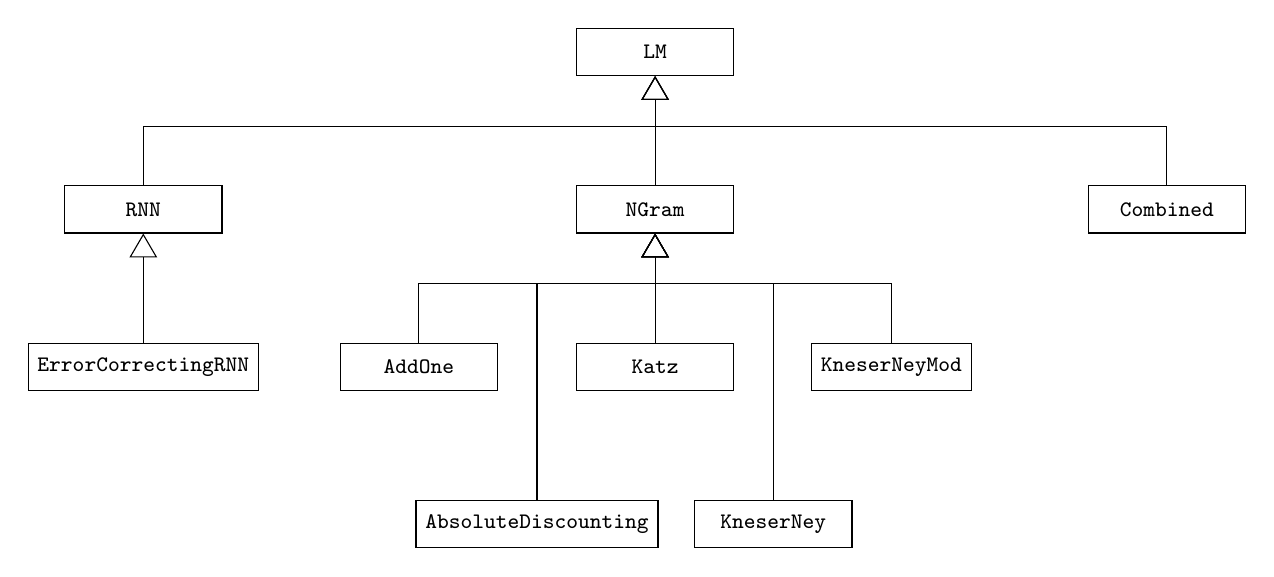
\begin{tikzpicture}[
		>=stealth,
		class/.style={draw, rectangle, minimum width=20mm, minimum height=6mm, align=center, font=\footnotesize},
	]
	\node[class] (lm) at (0,0) {\ttt{LM}};
	\node[class] (ngram) at (0, -2) {\ttt{NGram}};
	\node[class] (rnn) at (-6.5, -2) {\ttt{RNN}};
	\node[class] (combined) at (6.5, -2) {\ttt{Combined}};
	
	\node[class] (error_correcting) at (-6.5, -4) {\ttt{ErrorCorrectingRNN}};
	\node[class] (katz) at (0, -4) {\ttt{Katz}};
	\node[class] (add1) at (-3, -4) {\ttt{AddOne}};
	\node[class] (mkn) at (3, -4) {\ttt{KneserNeyMod}};
	\node[class] (abs) at (-1.5, -6) {\ttt{AbsoluteDiscounting}};
	\node[class] (kn) at (1.5, -6) {\ttt{KneserNey}};

	\foreach \i/\j in {ngram/lm, error_correcting/rnn, katz/ngram}
		\draw[-{Triangle[open, angle=60:10pt]}] (\i) -- (\j);

	\draw[-{Triangle[open, angle=60:10pt]}] (rnn.north) |- ++(10mm, 7.5mm) -| (lm.south);
	\draw[-{Triangle[open, angle=60:10pt]}] (combined.north) |- ++(-10mm, 7.5mm) -| (lm.south);

	\draw[-{Triangle[open, angle=60:10pt]}] (add1.north) |- ++(10mm, 7.5mm) -| (ngram.south);
	\draw[-{Triangle[open, angle=60:10pt]}] (mkn.north) |- ++(-10mm, 7.5mm) -| (ngram.south);
	\draw[-{Triangle[open, angle=60:10pt]}] (abs.north) |- ++(10mm, 27.5mm) -| (ngram.south);
	\draw[-{Triangle[open, angle=60:10pt]}] (kn.north) |- ++(-10mm, 27.5mm) -| (ngram.south);
\end{tikzpicture}
\caption{An outline of the C++ classes in the language model inheritance hierarchy. Methods and members are omitted for simplicity.}
\label{fig:hierarchy}
\end{figure}

For the RNN-based language models, the differences between the vanilla RNN, GRU and LSTM implementations arise in the Python code where the models are constructed and trained. The C++ code for the RNN-based models just loads and runs inference on the model graph described in the exported protocol buffer. See~\ref{tensorflow} for more details.

\subsection{Testing}

To encourage correctness, every non-trivial C++ and Python class in the codebase has an accompanying test class which contains one or more unit tests. In particular, the language model classes are paired with tests that query their \ttt{Prob()} and \ttt{ProbAllFollowing()} methods and compare the results with values that I calculated by hand using the equations presented in chapter~\ref{preparation}. \\

During the development of the project, all new code was tested before being committed to the codebase, and new test cases were immediately added upon discovery of any bugs.

\section{$n$-gram Models} \label{ngram_lm}

Below I detail my implementation of the $n$-gram models and their associated smoothing techniques. \\

One of the first things I discovered when implementing $n$-gram language models is that there is a trade-off between how much computation is done at training time, and how much computation is done at inference time. For example, at one extreme you could compute only the number of times each $n$-gram occurs at training time, and leave the computation of the coefficients in the smoothing equations to be calculated on the fly. At the other extreme, you could compute and store the final value of the probability for every possible $n$-gram that can be formed from the words in the language model vocabulary, and then return the relevant probability immediately at inference time. The problem with the first approach is that the language model would be too slow at inference time, and the problem with the second approach is that storing absolute probabilities for every possible $n$-gram would occupy far too much space to be practical. In my implementation, I try to strike a balance between these two extremes by precomputing and efficiently storing all of the relevant coefficients for the smoothing equations, and then combining them at inference time to compute the required $n$-gram probability. \\

\begin{figure}[h]
\captionsetup{justification=centering}
\centering
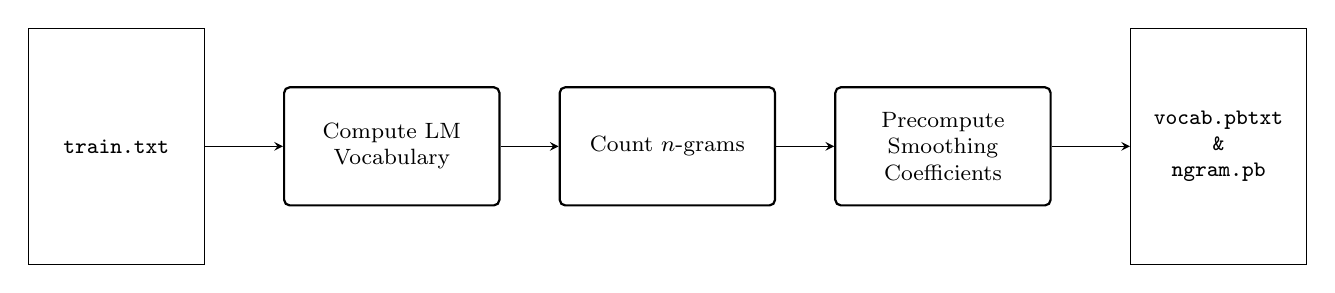
\begin{tikzpicture}[
		>=stealth,
		stage/.style={draw, rectangle, thick, rounded corners=2pt, minimum width=25mm, minimum height=15mm, text width=25mm, align=center, font=\footnotesize},
		file/.style={draw, rectangle, minimum width=20mm, minimum height=30mm, text width=20mm, align=center, font=\footnotesize\ttfamily},
	]
	\node[file] (training_set) at (0, 0) {\ttt{train.txt}};
	\node[stage] (vocab) at (3.5, 0) {Compute LM Vocabulary};
	\node[stage] (count) at (7, 0) {Count $n$-grams};
	\node[stage] (precompute) at (10.5, 0) {Precompute Smoothing Coefficients};
	\node[file] (ngram_proto) at (14, 0) {vocab.pbtxt\\ \& \\ ngram.pb};

	\draw[->] (training_set) -- (vocab);
	\draw[->] (vocab) -- (count);
	\draw[->] (count) -- (precompute);
	\draw[->] (precompute) -- (ngram_proto);
\end{tikzpicture}
\caption{The $n$-gram training pipeline.}
\label{fig:ngram_training}
\end{figure}

The three stages of my $n$-gram training pipeline are outlined in sections~\ref{ngram_compute_vocab}, \ref{ngram_count} and \ref{ngram_precompute} respectively.

\subsection{Computing the Vocabulary} \label{ngram_compute_vocab}

The first stage involves a single pass over \ttt{train.txt}, where words that occur at least $k$ times are added to the vocabulary and mapped to an integer ID. $k$ is called the \tit{minimum frequency}. A special marker \ttt{<unk>} is included in the vocabulary to represent any out-of-vocabulary words. That is, when the model encounters a word it has not seen before, it treats it as \ttt{<unk>}. The marker \ttt{<s>} is also included and is used to denote the end of a sentence.

\subsection{Counting $n$-grams Efficiently} \label{ngram_count}

For $n$-gram models without any smoothing, the only information that needs to be computed at this stage is $c(w_{i - n + 1}^{i})$ and $\sum_w c(w_{i - n + 1}^{i - 1}w)$, which are the number of times each $n$-gram $w_{i - n + 1}^i$ occurred in \ttt{train.txt}, and the sum of all such counts for all words that follow the $(n-1)$-gram $w_{i - n + 1}^{i - 1}$ respectively. Then, when the $n$-gram model is queried for the probability of $w_{i - n + 1}^i$, it can simply return the first number divided by the second, as required in equation~\ref{eq:ngram}. \\

This situation becomes more complex once smoothing techniques are included. For instance, absolute discounting requires the knowledge of $N_{1+}(w_{i - n + 1}^{i - 1}\bullet)$, the number of unique words that follow $w_{i - n + 1}^{i - 1}$, for every such $(n - 1)$-gram. Moreover, because it employs backoff, it actually requires this knowledge for every $k$-gram where $1 \leq k < n$. Kneser-Ney smoothing additionally requires $N_{1+}(\bullet w_{i - k + 1}^i)$, the number of unique words that precede $w_{i - k + 1}^i$, and $\sum_w N_{1+}(\bullet w_{i - k + 1}^iw)$, the number of unique pairs of words that follow and precede $w_{i - k + 1}^i$, for every $k$-gram where $1 \leq k < n$. \\

In my implementation, I precompute and store all of these parameters in a temporary word-level trie, as shown in figure~\ref{fig:count_trie}. This way, each parameter is only ever computed once and is accessible in $O(n)$ time. Given that I only consider $n$-grams for $n=2$, 3, 4 or 5, the access time practically constant.

\begin{figure}[h]
\captionsetup{justification=centering}
\centering
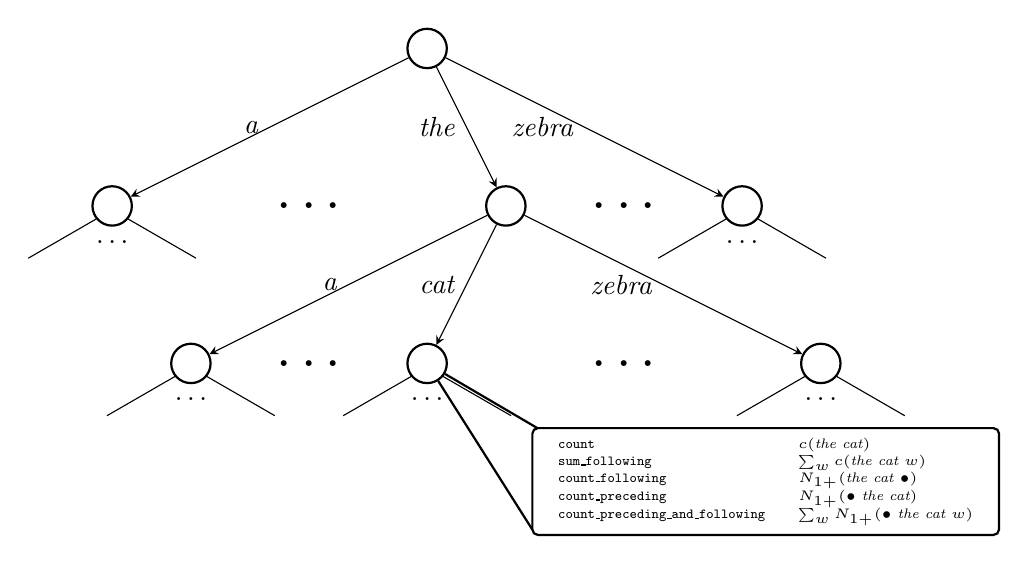
\begin{tikzpicture}[
		>=stealth,
		tnode/.style={draw, circle, thick, minimum width=5mm},
	]
	
	\node[tnode] (a1) at (0, 0) {};
	
	\node[tnode] (b1) at (-4, -2) {};
	\node[scale=2] (bvar1) at (-1.5, -2) {$\hdots$};
	\node[tnode] (b2) at (1, -2) {};
	\node[scale=2] (bvar2) at (2.5, -2) {$\hdots$};
	\node[tnode] (bk) at (4, -2) {};

	\node[tnode] (c1) at (-3, -4) {};
	\node[scale=2] (cvar1) at (-1.5, -4) {$\hdots$};
	\node[tnode] (c2) at (0, -4) {};
	\node[scale=2] (cvar2) at (2.5, -4) {$\hdots$};
	\node[tnode] (ck) at (5, -4) {};

	\draw[->] (a1) to node [left] {\tit{a}} (b1);
	\draw[->] (a1) to node [left] {\tit{the}} (b2);
	\draw[->] (a1) to node [left] {\tit{zebra}} (bk);

	\draw[->] (b2) to node [left] {\tit{a}} (c1);
	\draw[->] (b2) to node [left] {\tit{cat}} (c2);
	\draw[->] (b2) to node [left] {\tit{zebra}} (ck);

	\node[below=0.5mm of b1.south] {$\hdots$};
	\draw[-] ([xshift=-2mm, yshift=1mm]b1.south)--++(210:10mm);
	\draw[-] ([xshift=2mm, yshift=1mm]b1.south)--++(330:10mm);

	\node[below=0.5mm of c1.south] {$\hdots$};
	\draw[-] ([xshift=-2mm, yshift=1mm]c1.south)--++(210:10mm);
	\draw[-] ([xshift=2mm, yshift=1mm]c1.south)--++(330:10mm);

	\node[below=0.5mm of c2.south] {$\hdots$};
	\draw[-] ([xshift=-2mm, yshift=1mm]c2.south)--++(210:10mm);
	\draw[-] ([xshift=2mm, yshift=1mm]c2.south)--++(330:10mm);

	\node[below=0.5mm of bk.south] {$\hdots$};
	\draw[-] ([xshift=-2mm, yshift=1mm]bk.south)--++(210:10mm);
	\draw[-] ([xshift=2mm, yshift=1mm]bk.south)--++(330:10mm);

	\node[below=0.5mm of ck.south] {$\hdots$};
	\draw[-] ([xshift=-2mm, yshift=1mm]ck.south)--++(210:10mm);
	\draw[-] ([xshift=2mm, yshift=1mm]ck.south)--++(330:10mm);

	\node[draw, rectangle, rounded corners=2pt, thick, font=\tiny, fill=white] (inside) at (4.3, -5.5) {\begin{tabular}{l l} \ttt{count} & $c(\tit{the cat})$ \\ \ttt{sum\_following} & $\sum_w c(\tit{the cat }w)$ \\ \ttt{count\_following} & $N_{1+}(\tit{the cat }\bullet)$ \\ \ttt{count\_preceding} & $N_{1+}(\bullet \tit{ the cat})$ \\ \ttt{count\_preceding\_and\_following} &  $\sum_w N_{1+}(\bullet \tit{ the cat }w)$ \end{tabular}};

	\draw[-, thick] (c2) -- ([xshift=0.8mm, yshift=-0.15mm]inside.north west);
	\draw[-, thick] (c2) -- ([xshift=0.15mm, yshift=0.8mm]inside.south west);
\end{tikzpicture}
\caption{An example instance of the \ttt{CountTrie} class, which is the end result of the `Count $n$-grams' stage in figure~\ref{fig:ngram_training}.}
\label{fig:count_trie}
\end{figure}

Populating a \ttt{CountTrie} instance works in two phases. In the first phase, all of the $k$-grams, where $1 \leq k \leq n$, from the training set are inserted into the trie. At every insertion, the relevant \ttt{count} and \ttt{count\_preceding} values are updated. The second phase involves a full traversal of the trie in which the \ttt{sum\_following}, \ttt{count\_following} and \ttt{count\_following\_and\_preceding} values are computed. Each of these values can be derived for a particular node by looking at the \ttt{count} or \ttt{count\_preceding} values of its children. \\

It is worth noting that this data structure is temporary. That is, it is only used to enable fast computation of the smoothing coefficients in the next stage.

\subsection{Precomputing Smoothing Coefficients} \label{ngram_precompute}

With a few exceptions, most smoothing techniques can be generalised to the following form:
\begin{gather} \label{eq:smoothing_general}
	\mathbb{P}(w_i | w_{i - n + 1}^{i - 1})_{\text{\scshape SMOOTH}} = \alpha(w_{i - n + 1}^i) + \beta(w_{i - n + 1}^{i - 1})\mathbb{P}(w_i | w_{i - n + 2}^{i - 1})_{\text{\scshape SMOOTH}}
\end{gather}
The probabilities of many different $n$-grams share some of the same $\alpha$ and $\beta$ coefficients. For example, $\mathbb{P}(\tit{sat}\ |\ \tit{the cat})_{\text{\scshape SMOOTH}}$ and $\mathbb{P}(\tit{jumped}\ |\ \tit{the cat})_{\text{\scshape SMOOTH}}$ would both require $\beta(\tit{the cat})$. To avoid duplicated computation, the $\alpha$ and $\beta$ values for every $k$-gram in the \ttt{CountTrie} instance are computed exactly once and stored in a new word-level trie, called \ttt{ProbTrie}. Each node in this trie stores two values, $\alpha(w_i^j)$ and $\beta(w_i^j)$, where $w_i^j$ is the path of words that lead to the node. This way, the parameters can be fetched in $O(n)$ time at $n$-gram model query time, which again is practically constant since I only use $n \leq 5$. The \ttt{CountTrie} instance supplies the necessary parameters for deriving the smoothing coefficients used to populate the \ttt{ProbTrie} instance. \\

Once the \ttt{ProbTrie} instance has been populated, computing the probability of any $n$-gram can be done by traversing the data structure as shown in algorithm~\ref{alg:smoothing_prob}. Using this implementation, the only thing that each smoothing subclass has to override is the way in which the coefficients $\alpha$ and $\beta$ are calculated when the \ttt{ProbTrie} instance is initially populated. This made it much easier to add and test new smoothing techniques.

\begin{algorithm}
\caption{Computing $\mathbb{P}(w_i | w_{i - n + 1}^{i - 1})_{\text{\scshape SMOOTH}}$}
\label{alg:smoothing_prob}
\begin{algorithmic}[1]
\Procedure{Prob($w_i$, $w_{i - n + 1}^{i - 1}$)}{}
\If {$length(w_{i - n + 1}^i) > 0$}
	\State $node \gets \text{\scshape GetNode}(w_{i - n + 1}^i)$
	\State $\alpha \gets 0$
	\State $\beta \gets 1$
	\If {$node$}
		\State $\alpha \gets node.\alpha$
	\EndIf
	\If {$length(w_{i - n + 1}^{i - 1}) > 0$}
		\State $b\_node \gets \text{\scshape GetNode}(w_{i - n + 1}^{i - 1})$
		\If {$b\_node$}
			\State $\beta \gets b\_node.\beta$
		\EndIf
	\EndIf
	\State \Return $\alpha + (\beta \cdot \text{\scshape Prob}(w_i, w_{i - n + 2}^{i - 1}))$
\EndIf
\State \Return $0$
\EndProcedure
\end{algorithmic}
\end{algorithm}

Katz smoothing is an exception in that it does not quite match the form presented in equation~\ref{eq:smoothing_general}. To get around this issue, the Katz subclass simply overrides algorithm~\ref{alg:smoothing_prob} to traverse the same data structure in a slightly different way. \\

Once the \ttt{ProbTrie} instance is populated, it is exported to a protocol buffer in binary format, \ttt{ngram.pb}. The vocabulary is exported to a protocol buffer in textual format, \ttt{vocab.pbtxt}.

\section{Recurrent Neural Network Models} \label{rnn_lm}

Below, I explain how I implemented my RNN-based language models. To do this, I first give a brief overview of TensorFlow in section~\ref{tensorflow}. Then, in section~\ref{rnn_structure}, I explain the structure of the RNNs I use and how they apply to language modelling. In section~\ref{architectures} I give details of the GRU and LSTM architectures. Section~\ref{embeddings} describes the word embeddings used in the models. Finally, section~\ref{in_practice} outlines how I tuned the RNN hyperparameters and applied techniques to encourage convergence and avoid overfitting.

\subsection{TensorFlow} \label{tensorflow}

TensorFlow~\cite{tensorflow:abadi2016} is an open-source machine learning library that I used to implement my RNN-based language models. \\

Computation in TensorFlow is defined in terms of a directed graph, where each node represents an operation and each directed edge represents the flow of a tensor, hence the name. TensorFlow programs consist of two key sections: the first is constructing the graph, and the second is executing one or more paths through the graph in what is called a \tit{session}. In order to execute a path through a graph, you specify one or more nodes to evaluate, and then TensorFlow automatically executes all operations that are required to evaluate the tensor(s) at the specified node(s). \\

\begin{figure}[h]
\captionsetup{justification=centering}
\centering
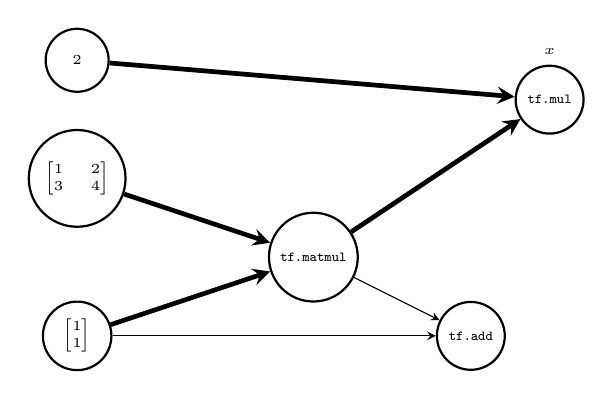
\begin{tikzpicture}[
		>=stealth,
		tfnode/.style={draw, circle, thick, minimum width=8mm, align=center, font=\tiny},
		thickl/.style={->, line width=0.6mm},
	]
	\node[tfnode] (a) at (0, 3.5) {$2$};
	\node[tfnode] (b) at (0, 2) {$\begin{bmatrix} 1 & 2 \\ 3 & 4 \end{bmatrix}$};
	\node[tfnode] (c) at (0, 0) {$\begin{bmatrix} 1 \\ 1 \end{bmatrix}$};
	\node[tfnode] (d) at (3, 1) {\ttt{tf.matmul}};
	\node[tfnode] (e) at (6, 3) {\ttt{tf.mul}};
	\node[above=0mm of e] (e_label) {\tiny $x$};
	\node[tfnode] (f) at (5, 0) {\ttt{tf.add}};
	
	\draw[thickl] (b) -- (d);
	\draw[thickl] (c) -- (d);
	\draw[thickl] (a) -- (e);
	\draw[thickl] (d) -- (e);
	\draw[->] (d) -- (f);
	\draw[->] (c) -- (f);
\end{tikzpicture}
\caption{A toy TensorFlow computation graph. On evaluation of node $x$, only the operations on the highlighted paths are computed, and 20 (a rank-0 tensor) is returned.}
\label{fig:tensorflow}
\end{figure}
Each operation takes zero or more tensors as input, and produces a tensor as output. There are some notable operations that take zero inputs: a \tit{constant}, which outputs a tensor whose value cannot be changed; a \tit{variable}, which is the same except the tensor that it outputs can be changed; and a \tit{placeholder}, which is a promise to provide a tensor at execution time. \\

In my implementation, I described my RNN-based language models as a directed graph of tensor operations. For example: layers of neurons were represented as a vectors and the weights in-between each layer were represented as a matrix. In the case of the vanilla RNN, I computed a layer of activations using the matrix operations presented in equation~\ref{eq:vanilla_rnn}. I used a \tit{placeholder} to provide the input training data, and \tit{variables} to store all of the trainable parameters of the network, namely the weights, bias variables and the word embeddings. \\

Once I constructed my RNN, I ran forward propagation through the network by evaluating the output nodes of the network in a \tit{session}. TensorFlow has a useful method called \ttt{tf.gradients(ys, xs)}, which returns the partial derivatives of the sum of the tensor(s) in \ttt{ys} with respect to the variables in \ttt{xs}. This is known as \tit{automatic differentiation}. By setting \ttt{xs} to the trainable parameters of the network and \ttt{ys} to the loss function, I avoided having to hard-code the backpropagation computation. Using these partial derivatives, I then applied an optimisation technique such as gradient descent to update the trainable parameters of the network. \\

After having trained the RNN in Python, I would \tit{freeze} the computation graph and export it into a format that can be loaded into C++. This involved converting all of the variables in the graph to constants and saving the network, along with some metadata, into a protocol buffer. Using the C++ API, I could then load the network and run inference on it by evaluating the relevant tensors in a session, without having to know anything about the internal structure of the RNN.

\subsection{Network Structure} \label{rnn_structure}

The general structure of all of my RNN-based language models is described below. \\

Before the RNN is constructed, an initial pass is made over the training set to construct a vocabulary $V$. This is done in exactly the same way as for the $n$-gram models, as described in section~\ref{ngram_compute_vocab}, so I will not repeat the detail. \\

At the very start of the network is a word embedding lookup table, that maps words to vectors that represent points in a high dimensional space. In my implementation, I set the number of vector elements in each word embedding to be the same as the number of hidden neurons in each hidden layer of the RNN. This is a configurable parameter, $H$, which was typically set to 256. \\

After the embedding lookup is the input layer of the RNN into which the word embeddings are fed. There are then two hidden layers which are recurrently connected to themselves, followed by the output layer. \\

There are $|V|$ neurons in the output layer, each of which represent a word in the language model vocabulary. Rather than feeding the logits of the output neurons through an activation function, they are passed through the softmax function. That is, if the vector of logits of the output neurons is denoted $\mathbf{z}$, then the output of neuron $j$ after the softmax function is defined as $\text{\scshape Softmax}(\mathbf{z})_j$, where:
\begin{gather}
	\text{\scshape Softmax}(\mathbf{z})_j = \frac{e^{z_j}}{\sum_i e^{z_i}}
\end{gather}
The outputs of the softmax function sum to 1 and are used to represent a probability distribution over all of the possible next words. That is, $\mathbb{P}(\text{next word} = j) = \text{\scshape Softmax}(\mathbf{z})_j$, where $j$ is the ID of a particular word in the vocabulary. Each ID lies in the range $[0, |V|)$.

\begin{figure}[h]
\captionsetup{justification=centering}
\centering
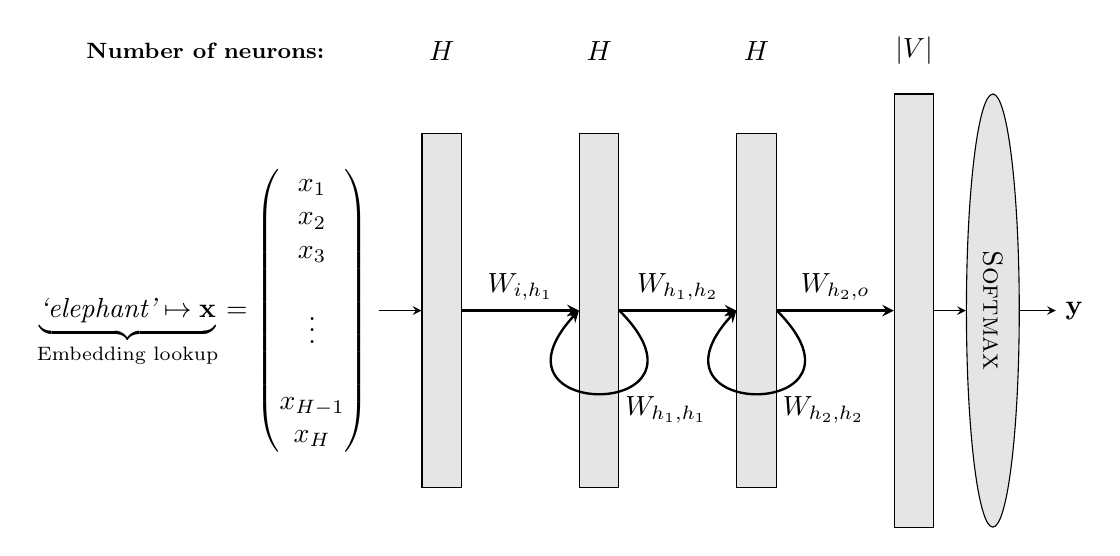
\begin{tikzpicture}[>=stealth]
	\node[draw, rectangle, minimum width=5mm, minimum height=45mm, fill=black!10, ] (input) at (0, 0) {};
	\node[draw, rectangle, minimum width=5mm, minimum height=45mm, fill=black!10] (hidden1) at (2, 0) {};
	\node[draw, rectangle, minimum width=5mm, minimum height=45mm, fill=black!10] (hidden2) at (4, 0) {};
	\node[draw, rectangle, minimum width=5mm, minimum height=55mm, fill=black!10] (output) at (6, 0) {};
	\node[draw, ellipse, minimum width=55mm, minimum height=5mm, fill=black!10, rotate=-90] (softmax) at (7, 0) {\scshape Softmax};

	\node at (-3, 3.3) {\footnotesize \tbf{Number of neurons:}};
	\node at (0, 3.3) {$H$};
	\node at (2, 3.3) {$H$};
	\node at (4, 3.3) {$H$};
	\node at (6, 3.3) {$|V|$};

	\draw [<-] (input) -- ++(-0.8, 0) node [left] {$\underbrace{\tit{`elephant'} \mapsto \mathbf{x}}_{\text{Embedding lookup}} = \begin{pmatrix} x_1 \\ x_2 \\ x_3 \\ \\ \vdots \\ \\ x_{H - 1} \\ x_H \end{pmatrix}$};
	\draw [->, line width=0.3mm] (input) to node [above] {$W_{i, h_1}$} (hidden1);
	\draw [->, line width=0.3mm] (hidden1) to node [above] {$W_{h_1, h_2}$} (hidden2);
	\draw [->, line width=0.3mm, out=-45, in=225, looseness=10] (hidden1.east) to node [below right=-1mm and 2mm of hidden1.east] {$W_{h_1, h_1}$} (hidden1.west);
	\draw [->, line width=0.3mm] (hidden2) to node [above] {$W_{h_2, o}$} (output);
	\draw [->, line width=0.3mm, out=-45, in=225, looseness=10] (hidden2.east) to node [below right=-1mm and 2mm of hidden2.east] {$W_{h_2, h_2}$} (hidden2.west);
	\draw [->] (output) -- (softmax);
	\draw [->] (softmax) -- ++(0.8, 0) node [right] {$\mathbf{y}$};
\end{tikzpicture}
\caption{The structure of my RNN-based language models.}
\end{figure}


\subsection{Long Short-Term Memory and Gated Recurrent Units} \label{architectures}

As mentioned in section~\ref{rnns}, there are various architectures that can be used for the neurons of RNNs, three of which I implemented in this project. Under the vanilla RNN architecture, a layer of neuron activations is computed as shown in equation~\ref{eq:vanilla_rnn}, which is repeated below. The fact that the vanilla RNN keeps hold of the activations of the hidden layers from the previous time step means that it implicitly maintains some state:
\begin{gather*}
	\mathbf{a}^{l, t} = \phi \big( \mathbf{W}^{l - 1} \mathbf{a}^{l - 1, t} + \mathbf{V}^l \mathbf{a}^{l, t - 1} + \mathbf{b}^{l - 1} \big)
\end{gather*}
Unfortunately, it is difficult to train vanilla RNNs to capture long-term dependencies, because the influence of the inputs as they cycle through the recurrent connections in the network often either decay or blow up exponentially~\cite{vanishing_gradient:hochreiter1991}~\cite{vanishing_gradient:bengio1994}, resulting in the weight gradients either vanishing or exploding disproportionately. These problems are known as the \tit{vanishing gradient problem} and the \tit{exploding gradient problem} respectively. Various RNN architectures have been constructed to improve upon these problems, two of which I implemented in my project and are outlined below.

\subsubsection{Long Short-Term Memory}

Hochreiter and Schmidhuber~\cite{lstm:hochreiter1997} originally proposed an architecture that directly tackles the vanishing gradient problem, called Long Short-Term Memory (LSTM). The state of each hidden layer $l$ in their architecture at time step $t$ consists of a tuple $(\mathbf{a}^{l, t}, \mathbf{c}^{l, t})$. $\mathbf{a}^{l, t}$, just like in the vanilla RNN cells, allows the LSTM cells to make decisions over a short period of time. The second state vector, $\mathbf{c}^{l, t}$, serves to retain longer-term information. At time step $t + 1$, each element $c_j^{l, t}$ of $\mathbf{c}^{l, t}$ passes through a single LSTM cell in layer $l$, and can be modified by a series of three \tit{gates}: the \tit{forget gate}, the \tit{input gate} and the \tit{output gate}. These gates can remove, add and output information respectively from $c_j^{l, t}$. \\

\begin{center}
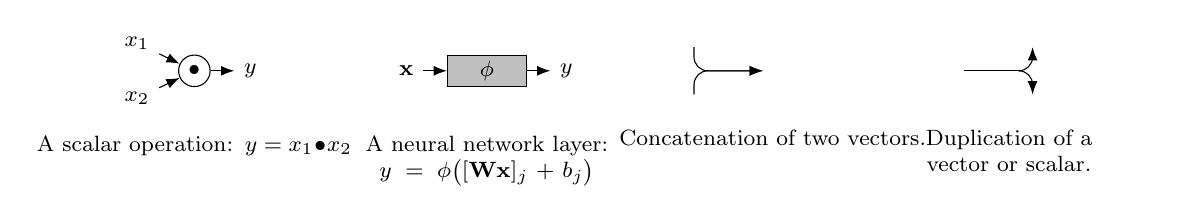
\begin{tikzpicture}[
	scalar/.style={circle, draw, inner sep=0pt, minimum width=4mm, font=\footnotesize},
	nnlayer/.style={rectangle, draw, inner sep=0pt, fill=gray!50, minimum width=10mm, minimum height=4mm, font=\footnotesize},
	textb/.style={minimum width=6mm, minimum height=4mm, text width=40mm, align=center, font=\footnotesize},
	>=LaTeX
]

\node[nnlayer] (nnlayer) {$\phi$};
\node[left=3mm of nnlayer] (nnlayer_input) {\footnotesize $\mathbf{x}$};
\node[right=3mm of nnlayer] (nnlayer_output) {\footnotesize $y$};
\node[textb, below=5mm of nnlayer] (nnlayertext) {A neural network layer: $y = \phi \big([\mathbf{W} \mathbf{x}]_j + b_j \big)$};

\node[scalar, left=30mm of nnlayer] (scalar) {$\bullet$};
\node[above left=0mm and 3mm of scalar] (scalar_input1) {\footnotesize $x_1$};
\node[below left=0mm and 3mm of scalar] (scalar_input2) {\footnotesize $x_2$};
\node[right=3mm of scalar] (scalar_output) {\footnotesize $y$};
\node[textb, below=5mm of scalar] (scalartext) {A scalar operation: $y = x_1 \bullet x_2$};

\node[right=30mm of nnlayer] (concat) {};
\node[textb, below=5mm of concat] (concattext) {Concatenation of two vectors.};

\node[right=60mm of nnlayer] (copy) {};
\node[textb, below=5mm of copy] (copytext) {Duplication of a vector or scalar.};

\draw[->] (nnlayer_input) -- (nnlayer);
\draw[->] (nnlayer) -- (nnlayer_output);

\draw[->] (scalar_input1) -- (scalar);
\draw[->] (scalar_input2) -- (scalar);
\draw[->] (scalar) -- (scalar_output);

\draw[<-, rounded corners=5pt] (concat) -| ++(-10mm,3mm);
\draw[<-, rounded corners=5pt] (concat) -| ++(-10mm,-3mm);

\draw[rounded corners=5pt] (copy.east) -- ++(-7mm,0mm);
\draw[->, rounded corners=5pt] (copy) -| ++(3mm,3mm);
\draw[->, rounded corners=5pt] (copy) -| ++(3mm,-3mm);

\end{tikzpicture}
\end{center}

In what follows, I use the notation from figure~\ref{fig:rnn_notation}, which is repeated above for convenience. Each LSTM gate has the following structure:

\begin{center}
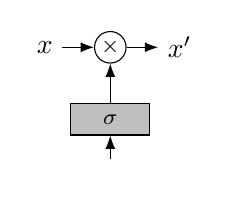
\begin{tikzpicture}[
	scalar/.style={circle, draw, inner sep=0pt, minimum width=4mm, font=\footnotesize},
	nnlayer/.style={rectangle, draw, inner sep=0pt, fill=gray!50, minimum width=10mm, minimum height=4mm, font=\footnotesize},
	textb/.style={minimum width=6mm, minimum height=4mm, text width=40mm, align=center, font=\footnotesize},
	>=LaTeX
]

\node[scalar] (times) {$\times$};
\node[left=4mm of times] (times_input) {$x$};
\node[right=4mm of times] (times_output) {$x'$};
\node[nnlayer, below=5mm of times] (sigmoid) {$\sigma$};
\node[below=3mm of sigmoid] (sigmoid_input) {};

\draw[->] (times_input) -- (times);
\draw[->] (times) -- (times_output);
\draw[->] (sigmoid_input) -- (sigmoid);
\draw[->] (sigmoid) -- (times);
\end{tikzpicture}
\end{center}
Each gate controls how much information from $x$ is let through to $x'$. The sigmoid layer outputs a scalar value in the range $[0, 1]$, where 0 prevents any information from $x$ passing through and 1 allows all of it to pass through. \\

\begin{figure}[h]
\captionsetup{justification=centering}
\centering
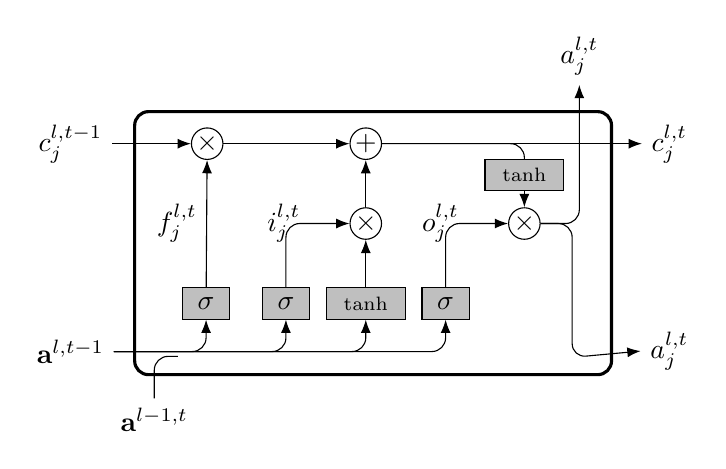
\begin{tikzpicture}[
	scalar/.style={circle, draw, inner sep=0pt, minimum width=4mm},
	tanlayer/.style={rectangle, draw, inner sep=0pt, fill=gray!50, minimum width=10mm, minimum height=4mm},
	siglayer/.style={rectangle, draw, inner sep=0pt, fill=gray!50, minimum width=6mm, minimum height=4mm},
	textb/.style={minimum width=6mm, minimum height=4mm},
	ct/.style={circle, draw, inner sep=5pt, ultra thick, minimum width=10mm},
	ft/.style={circle, draw, minimum width=8mm, inner sep=1pt},
	filter/.style={circle, draw, minimum width=7mm, inner sep=1pt, path picture={\draw[thick, rounded corners] (path picture bounding box.center)--++(65:2mm)--++(0:1mm);
	\draw[thick, rounded corners] (path picture bounding box.center)--++(245:2mm)--++(180:1mm);}},
	mylabel/.style={font=\scriptsize\sffamily},
	>=LaTeX
]

\node[scalar] (plus) {$+$};
\node[scalar, left=16mm of plus] (ftimes) {$\times$};
\node[scalar, below=6mm of plus] (itimes) {$\times$};
\node[scalar, right=16mm of itimes] (otimes) {$\times$};
\node[tanlayer, above=2mm of otimes] (otanh) {\scriptsize $\tanh$};
\node[tanlayer, below=6mm of itimes] (stanh) {\scriptsize $\tanh$};
\node[siglayer, left=2mm of stanh] (isig) {$\sigma$};
\node[siglayer, left=4mm of isig] (fsig) {$\sigma$};
\node[siglayer, right=2mm of stanh] (osig) {$\sigma$};
\node[textb, anchor=east, left=10mm of ftimes] (Cin) {$c_j^{l, t - 1}$};
\node[textb, anchor=east, below=20mm of Cin] (hin) {$\mathbf{a}^{l, t - 1}$};
\node[textb, anchor=west, right=33mm of plus] (Cout) {$c_j^{l, t}$};
\node[textb, anchor=west, below=19mm of Cout] (hout) {$a_j^{l, t}$};
\node[textb, anchor=north, below left=10mm and -2mm of fsig] (x) {$\mathbf{a}^{l - 1, t}$};
\node[textb, anchor=south, above right=6mm and 22mm of plus] (hout2) {$a_j^{l, t}$};
\node[left=5mm of itimes] {$i_j^{l, t}$};
\node[left=5mm of otimes] {$o_j^{l, t}$};
\node[below=2.5mm of stanh] (invisible) {};
\node[fit=(ftimes) (otanh) (osig) (fsig) (invisible), draw, inner xsep=6mm, inner ysep=2mm, rounded corners=5pt, line width=0.4mm] (fit) {};

\foreach \i/\j in {otimes/hout2, hin/fsig, hin/isig, hin/stanh, hin/osig}
	\draw[->, rounded corners=5pt] (\i) -| (\j);

\draw[-, rounded corners=5pt] (plus) -| (otanh);

\foreach \i/\j in {isig/itimes, osig/otimes}
	\draw[->, rounded corners=5pt] (\i) |- (\j);

\draw[->, rounded corners=5pt] (otimes.east) -| ++(4mm,-17mm) -- (hout.west);

\foreach \i/\j in {Cin/ftimes, ftimes/plus, plus/Cout, itimes/plus, stanh/itimes, otanh/otimes}
	\draw[->] (\i) -- (\j);

\draw[->] (fsig) to node [left] {$f_j^{l, t}$} (ftimes);

\draw[-, rounded corners=5pt] (x.north) |- ++(3mm, 5.34mm);

\end{tikzpicture}
\caption{A summary of the structure of an LSTM cell. Specifically, this diagram represents the computation of the $j^{th}$ cell in layer $l$ at time step $t$.}
\label{fig:lstm_structure}
\end{figure}

The LSTM forget, input and output gates in cell $j$ of layer $l$ at time step $t$ are denoted $f_j^{l, t}$, $i_j^{l, t}$ and $o_j^{l, t}$ respectively. If $[\mathbf{x}_1, \mathbf{x}_2]$ denotes the concatenation of vectors $\mathbf{x}_1$ and $\mathbf{x}_2$, and $[\mathbf{x}]_j$ denotes the $j^{th}$ element of vector $\mathbf{x}$, then the gate values are computed as follows:
\begin{align}
	f_j^{l, t} &= \sigma \big( [\mathbf{W}_f^l [\mathbf{a}^{l, t - 1}, \mathbf{a}^{l - 1, t}]]_j + [\mathbf{b}_f]_j \big) \\
	i_j^{l, t} &= \sigma \big( [\mathbf{W}_i^l [\mathbf{a}^{l, t - 1}, \mathbf{a}^{l - 1, t}]]_j + [\mathbf{b}_i]_j \big) \\
	o_j^{l, t} &= \sigma \big( [\mathbf{W}_o^l [\mathbf{a}^{l, t - 1}, \mathbf{a}^{l - 1, t}]]_j + [\mathbf{b}_o]_j \big)
\end{align}
Firstly, the forget gate determines how much of the long-term state value, $c_j^{l, t - 1}$, should be `forgotten'. Next, there is the opportunity for information derived from the short-term state, $\mathbf{a}^{l, t - 1}$, and the previous layer activation, $\mathbf{a}^{l - 1, t}$, to be added to the long-term state. The input gate decides how much of this information should be added. The application of the forget and input gates gives the new value of the long-term state value, $c_j^{l, t}$:
\begin{gather}
	c_j^{l, t} = f_j^{l, t} \cdot c_j^{l, t - 1} + i_j^{l, t} \cdot \tanh \big( [\mathbf{W}_c^l [\mathbf{a}^{l, t - 1}, \mathbf{a}^{l - 1, t}]]_j + [\mathbf{b}_c]_j \big)
\end{gather}
Finally, the output gate is used to control how much of the long-term state is used for the cell output, $a_j^{l, t}$:
\begin{gather}
	a_j^{l, t} = o_j^{l, t} \cdot \tanh (c_j^{l, t})
\end{gather}
This structure is summarised in figure~\ref{fig:lstm_structure}, and is the version of LSTM that I implemented in my project. There are many variants of LSTM, but I chose this one in particular because it represents a good baseline for the architecture. That is, most of the other versions are some form of extension of the one presented above, such as the notable use of \tit{peephole connections} from Gers and Schmidhuber~\cite{peephole:gers2000}.

\subsubsection{Gated Recurrent Unit}
Whilst the LSTM architecture provides a significant improvement for retaining long-term information, it is computationally expensive to run. Cho et al.\ propose the Gated Recurrent Unit~\cite{gru:cho2014}, which is a simplified version of LSTM that is cheaper to compute. The most significant changes are that it uses two gates rather than three, and it merges the long and short-term states into one. \\

\begin{figure}[h]
\captionsetup{justification=centering}
\centering
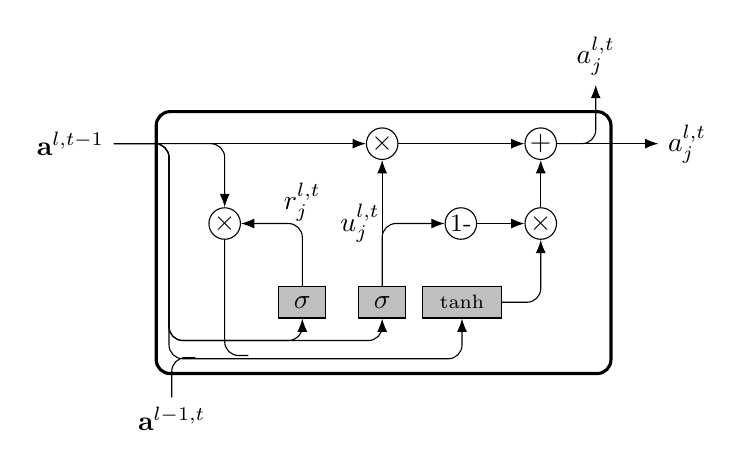
\begin{tikzpicture}[
	scalar/.style={circle, draw, inner sep=0pt, minimum width=4mm},
	tanlayer/.style={rectangle, draw, inner sep=0pt, fill=gray!50, minimum width=10mm, minimum height=4mm},
	siglayer/.style={rectangle, draw, inner sep=0pt, fill=gray!50, minimum width=6mm, minimum height=4mm},
	textb/.style={minimum width=6mm, minimum height=4mm},
	ct/.style={circle, draw, inner sep=5pt, ultra thick, minimum width=10mm},
	ft/.style={circle, draw, minimum width=8mm, inner sep=1pt},
	filter/.style={circle, draw, minimum width=7mm, inner sep=1pt, path picture={\draw[thick, rounded corners] (path picture bounding box.center)--++(65:2mm)--++(0:1mm);
	\draw[thick, rounded corners] (path picture bounding box.center)--++(245:2mm)--++(180:1mm);}},
	mylabel/.style={font=\scriptsize\sffamily},
	>=LaTeX
]

\node[scalar] (times) {$\times$};
\node[scalar, right=16mm of times] (plus) {$+$};
\node[scalar, below=6mm of plus] (times2) {$\times$};
\node[scalar, left=6mm of times2] (minus1) {\small 1-};
\node[scalar, left=36mm of times2] (times3) {$\times$};
\node[siglayer, below=16mm of times] (sig2) {$\sigma$};
\node[siglayer, left=4mm of sig2] (sig1) {$\sigma$};
\node[tanlayer, right=2mm of sig2] (tanh) {\scriptsize $\tanh$};
\node[textb, anchor=east, left=32mm of times] (hin) {$\mathbf{a}^{l, t - 1}$};
\node[textb, anchor=west, right=33mm of times] (hout) {$a_j^{l, t}$};
\node[textb, anchor=north, below left=10mm and 8mm of sig1] (x) {$\mathbf{a}^{l - 1, t}$};
\node[textb, anchor=south, above right=6mm and 22mm of times] (hout2) {$a_j^{l, t}$};
\node[below right=2.5mm and 17.5mm of sig2] (invisible) {};
\node[above=7mm of sig1] {$r_j^{l, t}$};
\node[left=7mm of minus1] {$u_j^{l, t}$};
\node[left=7mm of sig1] (invisible2) {};
\node[fit=(plus) (tanh) (invisible) (invisible2), draw, inner xsep=6mm, inner ysep=2mm, rounded corners=5pt, line width=0.4mm] (fit) {};

\foreach \i/\j in {hin/times3, plus/hout2, tanh/times2}
	\draw[->, rounded corners=5pt] (\i) -| (\j);

\foreach \i/\j in {sig1/times3, sig2/minus1}
	\draw[->, rounded corners=5pt] (\i) |- (\j);

\foreach \i/\j in {hin/times, times/plus, plus/hout, times2/plus, minus1/times2, sig2/times}
	\draw[->] (\i) -- (\j);

\foreach \i/\j in {hin.east/sig1.south, hin.east/sig2.south}
	\draw[->, rounded corners=5pt] (\i) -| ++(7mm,-25mm) -| (\j);

\draw[->, rounded corners=5pt] (hin.east) -| ++(7mm,-27.32mm) -| (tanh.south);

\draw[-, rounded corners=5pt] (times3.south) |- ++(3mm, -14.69mm);

\draw[-, rounded corners=5pt] (x.north) |- ++(3mm, 5.045mm);

\end{tikzpicture}
\caption{A summary of the structure of a GRU cell. Specifically, this diagram represents the computation of the $j^{th}$ cell in layer $l$ at time step $t$.}
\label{fig:gru_structure}
\end{figure}

The GRU consists of a \tit{reset gate}, $r_j^{l, t}$, and an \tit{update gate}, $u_j^{l, t}$:
\begin{align}
	r_j^{l, t} &= \sigma \big( [\mathbf{W}_r^l [\mathbf{a}^{l, t - 1}, \mathbf{a}^{l - 1, t}]]_j \big) \\
	u_j^{l, t} &= \sigma \big( [\mathbf{W}_u^l [\mathbf{a}^{l, t - 1}, \mathbf{a}^{l - 1, t}]]_j \big)
\end{align}
The cell output, $a_j^{l, t}$, is then computed as follows:
\begin{gather}
	a_j^{l, t} = u_j^{l, t} \cdot a_j^{l, t - 1} + (1 - u_j^{l, t}) \cdot \tilde{a}_j^{l, t}
\end{gather}
where
\begin{gather}
	\tilde{a}_j^{l, t} = \tanh \big( [\mathbf{W}_a^l [\mathbf{a}^{l, t - 1} \odot \mathbf{r}^{l, t}, \mathbf{a}^{l - 1, t}]]_j \big)
\end{gather}
and $\odot$ represents element-wise multiplication. \\

The reset gate acts similarly to the LSTM forget gate, in that it allows the cell to drop information that it deems irrelevant. The update gate controls how much information from the previous state carries over to the new one. With the short-term and long-term states combined into one, it follows that cells either learn to capture short or long-term information. Those that capture short-term information tend to have more active reset gates, whereas those that capture long-term information tend to have more active update gates.

\subsubsection{Abstraction Over the RNN Cells}

The LSTM architecture maintains 2-tuples of state vectors, whereas the vanilla RNN and GRU architectures only maintain 1-tuples. Apart from this, the three RNN cells only differ in how they are connected internally. I exploited this in my code by abstracting the implementation of each RNN cell from the overall network structure that was presented in section~\ref{rnn_structure}, so that new cell architectures could easily be added or tested.

\subsection{Word Embeddings} \label{embeddings}

As mentioned in section~\ref{rnn_structure}, each input word is first mapped to a vector representation known as a \tit{word embedding} which is learned as the network is trained. The aim is that similar words will be assigned points in the high-dimensional space which are closer together. This way, the RNN-based language model can more easily generalise to combinations of words that it has not seen before, by understanding which words can be substituted for one another. \\

In order to visualise such word embeddings, I used principle component analysis (PCA) to reduce the word embeddings to two-dimensional points that can be plotted on a scatter diagram. PCA is a dimensionality reduction technique that transforms the input data to a new coordinate system such that the first coordinate represents some projection that achieves the greatest variance, the second coordinate the second greatest variance, and so on.

\begin{figure}[h]
\captionsetup{justification=centering}
\centering
\begin{tikzpicture}[scale=1.25]
\begin{axis}
\addplot[only marks, fill=black, mark size=0.4] table [x=x, y=y, col sep=comma] {Data/embeddings_all.csv};

\draw[thick] (axis cs:0.6, -1.02) -- (axis cs:1.0, -1.02);
\draw[thick] (axis cs:1.0, -1.02) -- (axis cs:1.0, -1.3);
\draw[thick] (axis cs:1.0, -1.3) -- (axis cs:0.6, -1.3);
\draw[thick] (axis cs:0.6, -1.3) -- (axis cs:0.6, -1.02);

\draw[thick] (axis cs:-1.25, -1.3) -- (axis cs:-0.6, -1.3);
\draw[thick] (axis cs:-0.6, -1.3) -- (axis cs:-0.6, -2.7);
\draw[thick] (axis cs:-0.6, -2.7) -- (axis cs:-1.25, -2.7);
\draw[thick] (axis cs:-1.25, -2.7) -- (axis cs:-1.25, -1.3);
\end{axis}
\end{tikzpicture}
\caption{LSTM-based language model word embeddings projected onto two dimensions using PCA. The highlighted regions and are shown in figure~\ref{fig:pca_embeddings_zoomed}.}
\label{fig:pca_embeddings_all}
\end{figure}

The words that have been assigned a more distinguishable representation are given by the points which are further from the centre in figure~\ref{fig:pca_embeddings_all}.

\begin{figure}[h]
\captionsetup{justification=centering}
\centering
\begin{subfigure}{0.5\linewidth}
	\centering
	\centering
	\begin{tikzpicture}[scale=0.9]
	\begin{axis}[
		xmin=-1.35, xmax=-0.58,
		ymin=-2.7, ymax=-1.25]
	\addplot[only marks, fill=black, nodes near coords, point meta=explicit symbolic] table [x=x, y=y, col sep=comma, meta=w] {Data/embeddings_similar_to_should.csv};
	\end{axis}
	\end{tikzpicture}
	\caption{Words that express necessity, overlapping with a group of words that describe quantity.}
\end{subfigure}%
\begin{subfigure}{0.5\linewidth}
	\centering
	\begin{tikzpicture}[scale=0.9]
	\begin{axis}[
		xmin=0.62, xmax=1.0,
		ymin=-1.3, ymax=-1.02]
	\addplot[only marks, fill=black, nodes near coords, point meta=explicit symbolic] table [x=x, y=y, col sep=comma, meta=w] {Data/embeddings_similar_to_grew.csv};
	\end{axis}
	\end{tikzpicture}
	\caption{A group of words that characterise a dramatic change in value.}
\end{subfigure}
\caption{Two zoomed in regions of figure~\ref{fig:pca_embeddings_all}.}
\label{fig:pca_embeddings_zoomed}
\end{figure}

\subsection{Putting Theory into Practice} \label{in_practice}

In this section, I address a number of problems that are faced when training RNNs in practice and describe how I went about mitigating them.

\subsubsection{Underfitting and Overfitting}
In any supervised machine learning problem, there are one or more underlying patterns in the training data that need to be learned. \tit{Underfitting} occurs when the model fails to capture these patterns, and is typically the case when the model is too simple for the training data, or it is not trained for long enough. This problem was easy to mitigate by adding more parameters to the model, such as the number of hidden neurons, and training it for a sufficient amount of time. \\

As well as underlying patterns in the training data, there also often exists some noise which you do not want the model to learn. \tit{Overfitting} occurs when the model learns this noise, which makes it difficult for it to generalise to new data that it has not seen before. When each of my models were trained, a portion of the data called the test set was reserved for evaluating the performance of the model. The model was not allowed to see any of the data from the test set during training, so that its ability to generalise to unseen data was fairly assessed. In order to avoid overfitting my RNN-based language models, I also set aside a portion of data called the validation set. I used this to monitor, during training, the performance of my models on unseen data. As soon as this performance plateaued, I stopped the training process. \\

In my implementation, I evaluate the perplexity\footnote{Perplexity is the standard performance measure for language models, detailed in section~\ref{perplexity}.} of my language model on the validation set at the end of each training iteration. The learning rate starts at some initial value, $\eta_0$, and is then halved on every new iteration once the improvement of the perplexity on the validation set between two iterations drops below some threshold, $\Delta$. After this point, when the improvement of the perplexity on the validation set drops below 0.1\%, the training process is halted. I tried various values for $\eta_0$ and $\Delta$, and chose the best ones for each RNN architecture: $\eta_0 \in \{1, 0.5, 0.1, 0.01, 0.001\}$, $\Delta \in \{10\%, 5\%, 1\%, 0.5\%\}$. \\

RNNs with a large number of parameters can be particularly susceptible to overfitting. Srivastava proposes a technique called \tit{dropout} for reducing this problem~\cite{dropout:srivastava2013}, whereby some of the neurons and their connections are randomly dropped from the network during training. Zaremba et al.\ found that dropout works best in RNNs if it is only applied to the non-recurrent connections~\cite{dropout_rnns:zaremba2014}, which is the method I used in my RNN implementation.

\subsubsection{Convergence}
Whilst the LSTM and GRU architectures directly combat the aforementioned vanishing gradient problem, there is still the possibility that the gradients can explode, which can make the network unstable during training. In my implementation, I used \tit{gradient clipping} to mitigate this issue, whereby the gradients are clipped once their norm exceeds a certain threshold. \\

The selection of the initial learning rate value, $\eta_0$, was also important for ensuring convergence in my RNNs. If the learning rate is too large, then the weight updates may overshoot the minimum which they are directed towards. On the other hand, learning rates that are too small result in very slow convergence or the network becoming stuck in local minima.

\section{Mobile Keyboard} \label{mobile_keyboard}

As a project extension, I decided to apply one of my RNN-based language models in a practical context by building a mobile keyboard. \\

\begin{figure}[h]
\captionsetup{justification=centering}
\centering

\includegraphics[scale=0.25]{Images/MobileKeyboardOnScreen.png}
\caption{The mobile keyboard on iOS. The top three predictions are displayed at the top of the keyboard, and are updated with every character.}
\end{figure}

iOS applications are written in either Objective-C or Swift. An advantage of using Objective-C is that you can make use of Objective-C++ to link C++ code into your application, which is exactly what I needed to do. My C++ code, however, depended on TensorFlow, so in order to make my language models accessible within the mobile keyboard, I compiled both my RNN-language model implementation and a subset of TensorFlow's C++ API into a single static library by modifying one of the makefiles already present in the TensorFlow codebase. \\

To build a mobile keyboard in iOS, you have to implement what is called an `App Extension'. App Extensions differ from normal applications in iOS in that they their functionality is system-wide. Apple insist that such ubiquitous components should be extremely responsive and light-weight, which means that they have much stricter memory and CPU limitations than normal applications. Although they do not specify exactly what these limitations are, many people in the developer community estimate that the memory limit is approximately 30 MB. \\

In order to get an RNN-based language model to run under such memory and CPU limitations, I had to trade-off some of its prediction accuracy. In particular, I reduced the number of hidden layers, the number of hidden neurons and the size of the vocabulary to cut down both the CPU and memory pressure from the model at run time. The final model I used was a 1-layer vanilla RNN with 32 hidden neurons. I also removed the softmax layer, which is technically is not needed to rank the predictions, to further reduce the CPU overhead.

\subsection{Updating Language Model Predictions On the Fly}

A mobile keyboard should present the user with next-word predictions that are updated as they type. Querying the language model is a relatively expensive operation, so in my implementation I tried to do this as little as possible. For example, when the user presses the spacebar, I query the language model to retrieve the most probable words that could follow the space. These words are returned in the form of a character-level trie, where their associated probabilities are stored in the nodes of the trie. This way, when the user types subsequent characters, the new next-word predictions can be retrieved by traversing downwards from the root of the trie and taking the words with the highest probability on the current branch. \\

\section{Extending Models to Tackle Error-Prone Text} \label{error_correcting_lm}

An issue with existing language models is that their predictions suffer when presented with error-prone text. For example, consider the two word sequences `\tit{the weather is}' and `\tit{the whether is}'. Whilst in the first case a language model might successfully predict words such as `\tit{sunny}' or `\tit{nice}', in the second case it will likely struggle to suggest reasonable word candidates. Evidence to support this claim is given in figure~\ref{fig:error_correcting_results} in section~\ref{error_prone_evaluation}. \\

In the context of text prediction, it is unfortunately very rare that a human user will not make any mistakes. It is therefore an important issue to address and in this section I propose an extension to a language model which aims to improve its performance on text containing errors.

\subsection{The Approach}

My approach is to attack the source of the problem directly by adding a layer of error correction between the input text and the language model. There are lots of different types of error that can occur in the English language, but my implementation only focuses on correcting spelling mistakes. \\

Error-correction can be broken up into two parts: detecting the errors and making suggestions to fix them. In the case of spelling mistakes, detection can be done with a single dictionary lookup. Candidate corrections for a spelling mistake should be similar to the original word and probable in the surrounding context. In my implementation, I use the Levenshtein distance as a measure of how similar two words are, which is the minimum number of single character insertions, deletions and/or substitutions that need to be made to get from one word to the other. I also use the language model itself to gauge how probable candidate corrections are in the surrounding context. Specifically, when searching for candidate replacements for a word $w$ that is preceded by the words $w_i^j$, I feed $w_i^j$ to the language model, iterate through the next-word predictions in order of decreasing probability and select the first word that has an edit distance within some threshold $\delta$ of the original spelling, as described in algorithm~\ref{alg:error_correction}.

\begin{algorithm}
\caption{Computing $\mathbb{P}(w_j | w_i^{j - 1})_{\text{\scshape ERROR\_CORRECTING}}$}
\label{alg:error_correction}
\begin{algorithmic}[1]
\Procedure{Prob($w_j$, $w_i^{j - 1}$)}{}
\State $outputs \gets \emptyset$
\State $state = \mathbf{0}$
\For {$w$ in $w_i^{j - 1}$}
	\State $w_{correct} \gets w$
	\If {$w \notin dictionary\ \tbf{and}\ outputs \neq \emptyset$}
		\State $\text{\scshape SortByDecreasingProbability}(outputs)$
		\For {$w'$ in $outputs$}
			\State $d \gets \text{\scshape LevenshteinDistance}(w, w')$
			\If {$d \leq \delta$}
				\State $w_{correct} \gets w'$
				\State \textbf{break}
			\EndIf
		\EndFor
	\EndIf
	\State $outputs, state \gets \text{\scshape FeedForward}(w_{correct}, state)$
\EndFor
\State \Return $outputs[w_i]$
\EndProcedure
\end{algorithmic}
\end{algorithm}

I implemented this approach as an extension to my RNN-based language models, hence the use of {\scshape FeedForward}() and $state$.

\chapter{Evaluation} \label{evaluation}

In this chapter, I first describe the benchmarking framework that I built to evaluate the language models, before proceeding onto the results. The results section is threefold: firstly I present the performance of the existing language models that I implemented, secondly I focus on the tradeoffs faced when employing those models on a mobile device, and finally I display my findings in language modelling on error-prone text.

\section{Evaluation Methodology}

\subsection{Metrics} \label{metrics}

In the context of text prediction, there are essentially two questions one might want to answer when evaluating a language model:
\begin{align*}
	\tbf{Q1. } & \text{How accurately does the language model predict text?} \\
	\tbf{Q2. } & \text{How much resource, such as CPU or memory, does the language model consume?}
\end{align*}
I implemented a generic benchmarking framework that can return a series of metrics which are outlined below. The first two are concerned with \tbf{Q1} and the latter three relate to \tbf{Q2}.

\subsubsection{Perplexity} \label{perplexity}

Perplexity is the most widely-used metric for language models, and is therefore an essential one to include so that my results can be compared with those of other authors. Given a sequence of words $w_1^{N} = w_1w_2...w_N$ as test data, the perplexity PP of a language model $L$ is defined as:
\begin{gather} \label{eq:perplexity}
	\text{PP}_L(w_1^N) = \sqrt[N]{\frac{1}{\mathbb{P}_L(w_1^N)}} = \sqrt[N]{\prod_{i=1}^{N}\frac{1}{\mathbb{P}_L(w_i | w_1^{i-1})}}
\end{gather}
where $\mathbb{P}_L(w_i | w_1^{i-1})$ is the probability computed by the language model $L$ of the word $w_i$ following the words $w_1^{i-1}$. This somewhat arbitrary-looking formulation is more thoroughly justified with a bit of information theory in appendix~\ref{appendix:perplexity}. The key point is that \tit{lower values of perplexity indicate better prediction accuracy} for language models trained on a particular training set. \\

One issue with perplexity is that it is undefined if $\mathbb{P}_L(w_i | w_1^{i-1})$ is 0 at any point. In my implementation, I replaced probability values of 0 with the small constant \ttt{1e-9}. Results that use this approximation are marked.

\subsubsection{Average-Keys-Saved}

Average-keys-saved is a more user-oriented metric, which is defined as the number of characters that they can avoid typing as a result of the correct next words appearing in the top three predictions, averaged over the number of characters in the test data. As an example, if the user is typing \ttt{science} and the word \ttt{science} appears in the top three predictions after they have typed \ttt{sc}, then that would count as 5 characters being saved, averaging at $\frac{5}{7}$ keys saved per character. Averaging over the number of characters ensures that the results are not biased by having longer words in the test data.

\subsubsection{Memory Usage}

This is measured as the amount of physical memory in megabytes occupied by the process running the language model.

\subsubsection{Training Time}

The amount of time it took to train the language model.

\subsubsection{Average Inference Time}

This is measured as the amount of time in milliseconds that the language model takes to assign a probability to all of the words in its vocabulary given a sequence of words, averaged over a large number of sequences.

\subsection{Datasets}

\subsubsection{Penn Tree Bank (PTB) Dataset}

The Penn Tree Bank is a widely-adopted dataset for measuring the quality of language models, derived from text from the Wall Street Journal. The training set has 10,000 unique words and 887,521 words overall. I used it for all tests in which the size of the training data is fixed, and will refer to it as PTB.

\subsubsection{One Billion Word (1BW) Benchmark}

This is a much larger dataset produced by Google of approximately 1 billion words~\cite{1bw:chelba2013}. I used this dataset for tests in which the size of the training data is a variable under investigation, and will refer to it as 1BW.

\subsubsection{Cambridge Learner Corpus (CLC)}

The Cambridge Learner Corpus is a dataset of 1,244 exam scripts written by candidates sitting the Cambridge ESOL First Certificate in English examination in 2000 and 2001~\cite{clc:yannakoudakis2011}. In this project I make use of a preprocessed version of this dataset, in which error-prone and error-free versions of the exam scripts are aligned line by line in separate files. I used this dataset when exploring the performance of language models on error-prone text, and will refer to it as CLC.

\section{Results}

\subsection{Existing Models}

\subsubsection*{Smoothing techniques and the value of $n$ in $n$-gram models}

The first set of language models that I built were $n$-gram models, along with a series of smoothing techniques for improving their predictions on less frequent $n$-grams.

\begin{figure}[h]
\centering
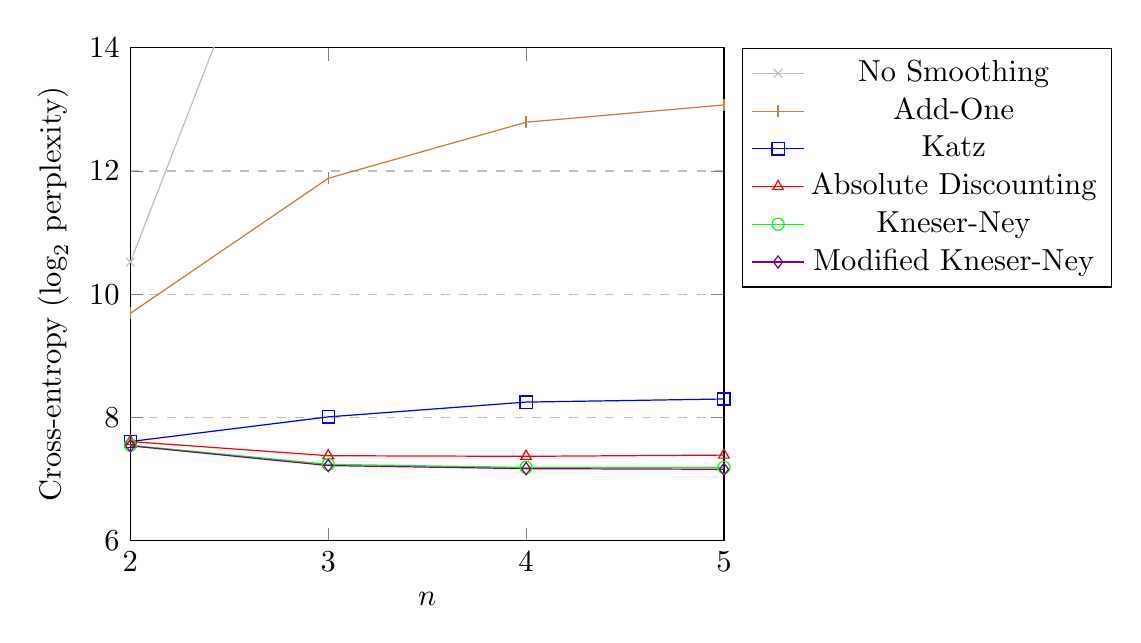
\begin{tikzpicture}[scale=1.1]
\begin{axis}[
	xlabel={$n$},
	ylabel={Cross-entropy ($\log_2$ perplexity)},
	xmin=2, xmax=5,
	ymin=6, ymax=14,
	xtick={2, 3, 4, 5},
	ytick={6, 8, 10, 12, 14},
	legend pos=outer north east,
	ymajorgrids=true,
	grid style=dashed,
]

\addplot[color=lightgray, mark=x]
coordinates {(2, 10.52)(3, 18.79)(4, 24.95)(5, 27.55)};

\addplot[color=brown, mark=|]
coordinates {(2, 9.69)(3, 11.88)(4, 12.79)(5, 13.07)};

\addplot[color=blue, mark=square]
coordinates {(2, 7.61)(3, 8.01)(4, 8.25)(5, 8.30)};

\addplot[color=red, mark=triangle]
coordinates {(2, 7.61)(3, 7.38)(4, 7.37)(5, 7.39)};

\addplot[color=green, mark=o]
coordinates {(2, 7.55)(3, 7.24)(4, 7.19)(5, 7.19)};

\addplot[color=violet, mark=diamond]
coordinates {(2, 7.54)(3, 7.22)(4, 7.17)(5, 7.16)};

\legend{No Smoothing, Add-One, Katz, Absolute Discounting, Kneser-Ney, Modified Kneser-Ney}
 
\end{axis}
\end{tikzpicture}
\caption{The cross-entropy of $n$-gram models trained on the PTB dataset.}
\end{figure}

Cross-entropy is the binary logarithm of perplexity, and lower perplexity scores indicate better prediction accuracy. With this in mind, it is clear that modified Kneser-Ney smoothing offers the best prediction performance amongst the $n$-gram models. \\

The change in performance with the value of $n$ is interesting, because one might expect that increasing $n$ will always yield better results. For $n$-gram models with add-one or no smoothing, this is not the case, because they do not employ backoff. At higher values of $n$, $n$-grams are much more sparse, so without any backoff these models can only rely on sparse counts, resulting is lower probabilities being assigned to plausible sequences of words. Katz smoothing does employ backoff, and achieves much better performance, but it still distributes too much probability to rare $n$-grams, which is why its performance also drops with $n$.

\subsubsection*{A comparison of RNN-based models with $n$-gram models}

I also implemented three RNN-based language models which differ in their cell architecture: vanilla RNN, Gated Recurrent Unit and Long Short-Term Memory. \\

\begin{figure}[h]
\captionsetup{justification=centering}
\centering
\begin{subfigure}{0.5\linewidth}
	\centering
	\begin{tabular}{L{7cm}}
		\hline
		\tbf{money is the root of} a new york city. \\ \hline
		\tbf{the meaning of life is} a unit of the company's shares outstanding. \\ \hline
		\tbf{science} and was up N N from \$ N million or N cents a share. \\ \hline
	\end{tabular}
	\caption{5gram + modified Kneser-Ney smoothing}
\end{subfigure}%
\begin{subfigure}{0.5\linewidth}
	\centering
	\begin{tabular}{L{7cm}}
		\hline
		\tbf{money is the root of} the nation's largest public bank. \\ \hline
		\tbf{the meaning of life is} the best way to get the way to the public. \\ \hline
		\tbf{science}'s most recent issue of the nation's largest economic indicators. \\ \hline
	\end{tabular}
	\caption{2-layer LSTM with 256 hidden neurons}
\end{subfigure}
\caption{Sentences generated from two different language models trained on the PTB dataset. The bold words were given to the model, and the non-bold words were generated until a full stop was predicted.}
\label{fig:generated_sentences}
\end{figure}

At a qualitative level it can be seen that the RNN-based language models are better at making predictions with long-term word dependencies than the $n$-gram smoothed models. This is demonstrated in figure~\ref{fig:generated_sentences}, and confirmed by the readings in figure~\ref{fig:cross_entropy_training_set_size}. \\

\begin{figure}[h]
\captionsetup{justification=centering}
\centering
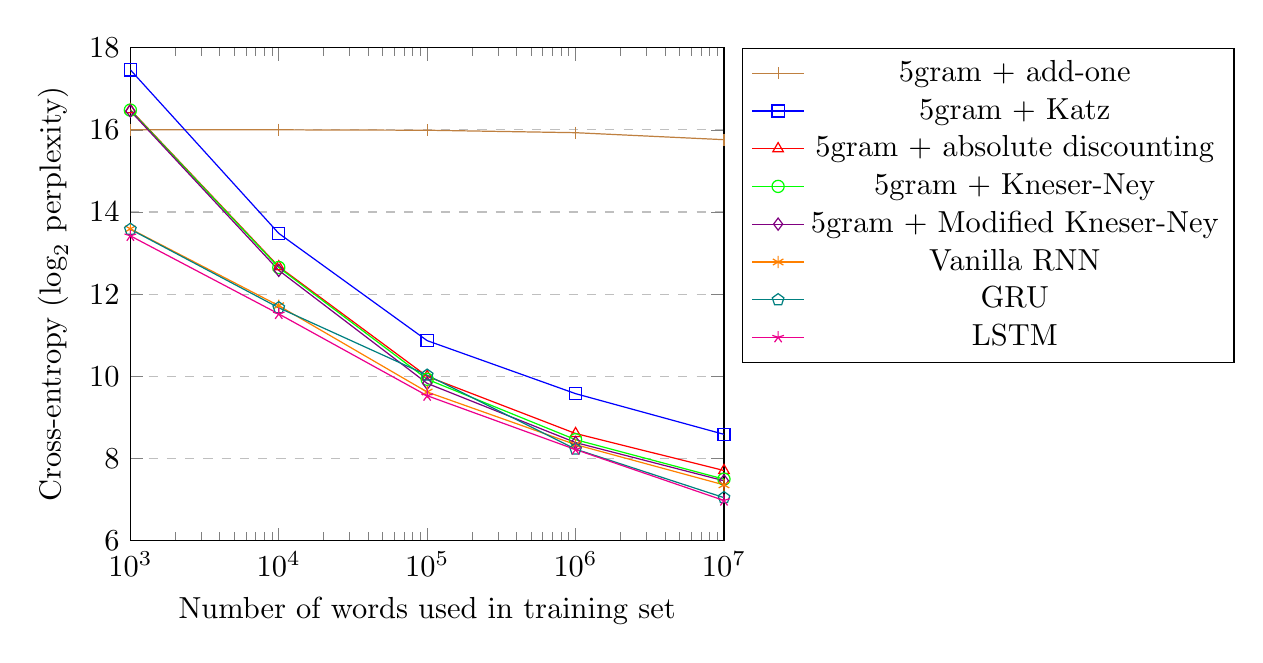
\begin{tikzpicture}[scale=1.1]
\begin{semilogxaxis}[
	xlabel={Number of words used in training set},
	ylabel={Cross-entropy ($\log_2$ perplexity)},
	xmin=1e3, xmax=1e7,
	ymin=6, ymax=18,
	legend pos=outer north east,
	ymajorgrids=true,
	grid style=dashed,
]

% 3gram
%\addplot[color=lightgray, mark=x]
%coordinates {(1e3, 29.33)(1e4, 28.22)(1e5, 25.58)(1e6, 21.29)(1e7, 16.25)};

% 3gram + add-one
%\addplot[color=brown, mark=|]
%coordinates {(1e3, 15.97)(1e4, 15.87)(1e5, 15.59)(1e6, 14.93)(1e7, 13.77)};

% 3gram + Katz
%\addplot[color=blue, mark=square]
%coordinates {(1e3, 17.40)(1e4, 13.48)(1e5, 10.83)(1e6, 9.28)(1e7, 8.14)};

% 3gram + absolute discounting
%\addplot[color=red, mark=triangle]
%coordinates {(1e3, 16.46)(1e4, 12.61)(1e5, 9.92)(1e6, 8.54)(1e7, 7.68)};

% 3gram + Kneser-Ney
%\addplot[color=green, mark=o]
%coordinates {(1e3, 16.45)(1e4, 12.60)(1e5, 9.85)(1e6, 8.41)(1e7, 7.54)};

% 3gram + modified Kneser-Ney
%\addplot[color=violet, mark=diamond]
%coordinates {(1e3, 16.46)(1e4, 12.58)(1e5, 9.84)(1e6, 8.40)(1e7, 7.53)};

% 5gram
%\addplot[color=lightgray, mark=x]
%coordinates {(1e3, 29.89)(1e4, 29.83)(1e5, 29.58)(1e6, 28.86)(1e7, 27.10)};

% 5gram + add-one
\addplot[color=brown, mark=|]
coordinates {(1e3, 16.00)(1e4, 16.00)(1e5, 15.99)(1e6, 15.93)(1e7, 15.76)};

% 5gram + Katz
\addplot[color=blue, mark=square]
coordinates {(1e3, 17.46)(1e4, 13.48)(1e5, 10.87)(1e6, 9.58)(1e7, 8.59)};

% 5gram + absolute discounting
\addplot[color=red, mark=triangle]
coordinates {(1e3, 16.49)(1e4, 12.67)(1e5, 10.00)(1e6, 8.61)(1e7, 7.71)};

% 5gram + Kneser-Ney
\addplot[color=green, mark=o]
coordinates {(1e3, 16.48)(1e4, 12.65)(1e5, 9.93)(1e6, 8.46)(1e7, 7.50)};

% 5gram + modified Kneser-Ney
\addplot[color=violet, mark=diamond]
coordinates {(1e3, 16.46)(1e4, 12.58)(1e5, 9.83)(1e6, 8.39)(1e7, 7.46)};

% Vanilla RNN 256
\addplot[color=orange, mark=asterisk]
coordinates {(1e3, 13.59)(1e4, 11.72)(1e5, 9.62)(1e6, 8.34)(1e7, 7.36)};

% GRU 256
\addplot[color=teal, mark=pentagon]
coordinates {(1e3, 13.58)(1e4, 11.67)(1e5, 10.03)(1e6, 8.23)(1e7, 7.05)};

% LSTM 256
\addplot[color=magenta, mark=star]
coordinates {(1e3, 13.42)(1e4, 11.52)(1e5, 9.53)(1e6, 8.22)(1e7, 6.98)};

\legend{
%	3gram, 3gram + add-one, 3gram + Katz, 3gram + absolute discounting, 3gram + Kneser-Ney, 3gram + Modified Kneser-Ney,
	5gram + add-one, 5gram + Katz, 5gram + absolute discounting, 5gram + Kneser-Ney, 5gram + Modified Kneser-Ney,
	Vanilla RNN, GRU, LSTM,
}
 
\end{semilogxaxis}
\end{tikzpicture}
\caption{The cross-entropy of various language models with respect to the training set size, using the 1BW dataset.}
\label{fig:cross_entropy_training_set_size}
\end{figure}

As can be seen in figure~\ref{fig:cross_entropy_training_set_size}, the RNN-based language models consistently outperform the $n$-gram based models in terms of prediction accuracy. This difference is most significant for small training sets, and starts to become more pronounced again once the training set grows large beyond $10^6$ words. \\

Some datasets are more predictable than others, which means that metrics like perplexity and average-keys-saved depend on which dataset is used. In order to produce results that are comparable with the work of other authors, I have tested my language models on the Penn Tree Bank dataset, as shown in figure~\ref{fig:ptb}. The RNN-based models used 2 hidden layers each with 256 neurons. The perplexity was calculated over the whole of the test set, whereas average-keys-saved, a more expensive metric to compute, was taken over the first 1000 words of the test set. \\

\begin{figure}[h]
\begin{adjustbox}{center}
\begin{tabular}{| L{5.2cm} | C{2.2cm} | C{2cm} | C{2cm} |  C{2cm} | C{2cm} |}
	\hline
	\tbf{Language Model} & \tbf{Perplexity} & \tbf{Average-Keys-Saved} & \tbf{Memory Usage (MB)} & \tbf{Training Time (min,secs)}$^\dagger$ & \tbf{Average Inference Time (ms)} \\ \hline
	3-gram & 4.54 $\times 10^5$$^*$ & 0.35014 & 266.91 & \tbf{11s} & 62 \\
	3-gram + add-one & 3764.96 & 0.53063 & 266.94 & \tbf{11s} & 41 \\
	3-gram + Katz & 256.95 & 0.68482 & 266.71 & 14s & 88 \\
	3-gram + absolute disc. & 166.03 & 0.72178 & 266.78 & 13s & 63 \\
	3-gram + KN & 150.73 & 0.72466 & 266.88 & 14s & 54 \\
	3-gram + modified KN & 149.54 & 0.72355 & 266.97 & 14s & 54 \\
	5-gram & 1.96 $\times 10^8$$^*$ & 0.07167 & 737.36 & 26s & 130 \\
	5-gram + add-one & 8610.45 & 0.33886 & 737.30 & 26s & 63 \\
	5-gram + Katz & 314.49 & 0.67154 & 737.43 & 41s & 156 \\
	5-gram + absolute disc. & 167.38 & 0.72333 & 737.43 & 40s & 126 \\
	5-gram + KN & 146.35 & 0.72598 & 737.37 & 44s & 114 \\
	5-gram + modified KN & 142.68 & 0.72554 & 737.53 & 50s & 116 \\ \hline
	Vanilla RNN & 131.03 & 0.72776 & \tbf{253.67} & 15m 10s & 39 \\
	Gated Recurrent Units & 114.52 & 0.73993 & 271.39 & 28m 35s & \tbf{37} \\
	Long Short-Term Memory & 112.47 & 0.73617 & 287.13 & 18m 59s & 38 \\ \hline
	LSTM, 5-gram\ +\ MKN (av) & 96.07 & 0.75719 & 929.39 & 19m 49s & 189  \\
	LSTM, 5-gram\ +\ MKN (int) & \tbf{94.70} & \tbf{0.75830} & 927.20 & 19m 49s & 190 \\ \hline
\end{tabular}
\end{adjustbox}
\begin{center}
	{\footnotesize\tit{$^*$These perplexity scores use the approximation mentioned in section \ref{metrics}. $^\dagger$The $n$-gram models were trained on my laptop, whereas the neural models were trained on a GPU cluster on the High Performance Computing service.}}
\end{center}
\caption{A benchmark of various language models on the PTB dataset.}
\label{fig:ptb}
\end{figure}

There is a lot of information that can be drawn from figure~\ref{fig:ptb}, so I will highlight only the most important and interesting points:
\begin{itemize}
\item
	The RNN-based language models outperform the $n$-gram models in terms of prediction accuracy. In my implementation, they run slightly faster at inference time and also consume less memory, although this is partly due to the fact that the $n$-gram models are entirely unpruned. The RNN-based language models, however, take significantly longer to train and obtain the correct hyperparameters for.
\item
	Ignoring insignificant differences in memory and time, absolute discounting, Kneser-Ney smoothing and modified Kneser-Ney smoothing equal or outperform add-one and Katz smoothing in every metric.
\item
	LSTM yields marginally better prediction accuracy than the GRU architecture, but requires more memory. Apart from the memory overhead, GRUs significantly outperform the vanilla RNN architecture. The differences in training time for the RNN-based models should be taken lightly, because each model was trained for a different number of iterations, depending on how long it took to converge to a steady perplexity score on the validation set.
\item
	Interestingly, a substantial improvement in perplexity and average-keys-saved can be obtained by simply averaging the probabilities produced by an $n$-gram and an RNN-based language model. This seems to imply that the two classes of language model complement one another, in the sense that RNN-based models make strong predictions when some of the $n$-gram predictions are weak, and vice versa.
\item
	The combined language models can be improved even more by interpolating their probabilities rather than just averaging them. The result shown for the interpolation of 5-gram modified Kneser-Ney with LSTM used $\lambda = 0.38$, where the probability was calculated as $\lambda$($n$-gram probability) + (1 - $\lambda$)(LSTM probability).
\end{itemize}

\subsection{On a Mobile Device}

The strict memory and CPU limitations I faced when implementing the mobile keyboard forced me to explore the tradeoffs between resource consumption and prediction performance. \\

Two obvious ways of decreasing the memory footprint of a language model are decreasing the vocabulary size and, for RNN-based models, decreasing the number of hidden neurons. What is less obvious, is how quickly the average-keys-saved drops with these two parameters. \\

\begin{figure}[h]
\captionsetup{justification=centering}
\centering
\begin{subfigure}{0.5\linewidth}
	\centering
	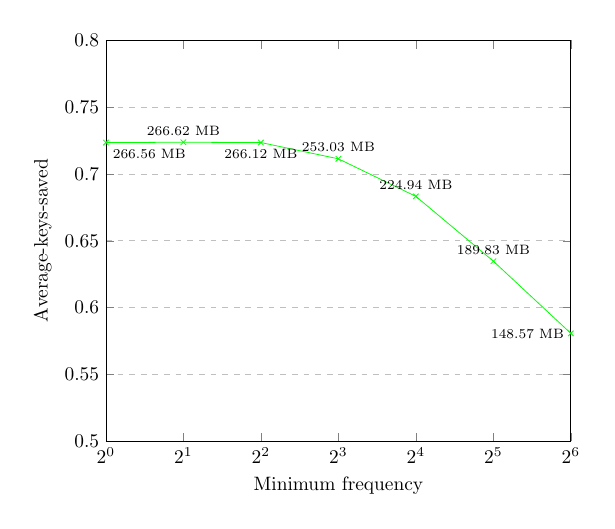
\begin{tikzpicture}[scale=0.7]
	\begin{semilogxaxis}[
		scale only axis,
		xmin=1,xmax=64,
		log basis x=2,
		xtick={1, 2, 4, 8, 16, 32, 64},
		ymin=0.5,ymax=0.8,
		ymajorgrids=true,
		grid style=dashed,
		xlabel=Minimum frequency,
		ylabel=Average-keys-saved]

		\addplot[color=green, mark=x]
		coordinates {(1, 0.72355)(2, 0.72377)(4, 0.72355)(8, 0.71138)(16, 0.68327)(32, 0.63479)(64, 0.58079)};

		\node [below right] at (axis cs:  1, 0.72355) {\scriptsize 266.56 MB};
		\node [above] at (axis cs:  2, 0.72377) {\scriptsize 266.62 MB};
		\node [below] at (axis cs:  4, 0.72355) {\scriptsize 266.12 MB};
		\node [above] at (axis cs:  8, 0.71138) {\scriptsize 253.03 MB};
		\node [above] at (axis cs:  16, 0.68327) {\scriptsize 224.94 MB};
		\node [above] at (axis cs:  32, 0.63479) {\scriptsize 189.83 MB};
		\node [left] at (axis cs:  64, 0.58079) {\scriptsize 148.57 MB};

	\end{semilogxaxis}	
	\end{tikzpicture}
	\caption{3gram + modified Kneser-Ney smoothing}
\end{subfigure}%
\begin{subfigure}{0.5\linewidth}
	\centering
	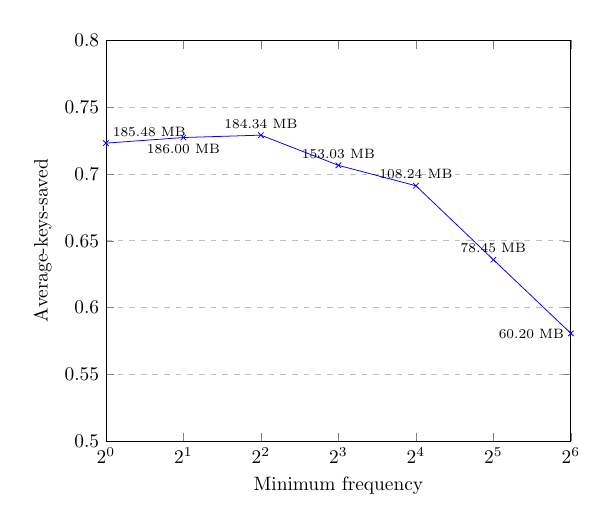
\begin{tikzpicture}[scale=0.7]
	\begin{semilogxaxis}[
		scale only axis,
		xmin=1,xmax=64,
		log basis x=2,
		xtick={1, 2, 4, 8, 16, 32, 64},
		ymin=0.5,ymax=0.8,
		ymajorgrids=true,
		grid style=dashed,
		xlabel=Minimum frequency,
		ylabel=Average-keys-saved]
		
		\addplot[color=blue, mark=x]
		coordinates {(1, 0.72311)(2, 0.72731)(4, 0.72908)(8, 0.70651)(16, 0.69124)(32, 0.63590)(64, 0.58079)};
		
		\node [above right] at (axis cs:  1, 0.72311) {\scriptsize 185.48 MB};
		\node [below] at (axis cs:  2, 0.72731) {\scriptsize 186.00 MB};
		\node [above] at (axis cs:  4, 0.72908) {\scriptsize 184.34 MB};
		\node [above] at (axis cs:  8, 0.70651) {\scriptsize 153.03 MB};
		\node [above] at (axis cs:  16, 0.69124) {\scriptsize 108.24 MB};
		\node [above] at (axis cs:  32, 0.63590) {\scriptsize 78.45 MB};
		\node [left] at (axis cs:  64, 0.58079) {\scriptsize 60.20 MB};
		
	\end{semilogxaxis}
	\end{tikzpicture}
	\caption{Vanilla RNN with 256 hidden neurons}
\end{subfigure}
\caption{The effect of the vocabulary size on average-keys-saved and memory usage for models trained on the PTB dataset.}
\end{figure}

The vocabulary size was altered by changing a parameter called the \tit{minimum frequency}, which defines the minimum number of times a word must appear in the training set to be considered part of the language model vocabulary. \\

For both the $n$-gram and vanilla RNN models, the minimum frequency can be increased to approximately $2^4$ before the average-keys-saved starts dropping rapidly. At this point, a saving of 77.24 MB is made in the vanilla RNN model, with a drop of only 0.03187 in average-keys-saved. The savings made on the $n$-gram model are less substantial. \\

\begin{figure}[h]
\captionsetup{justification=centering}
\centering
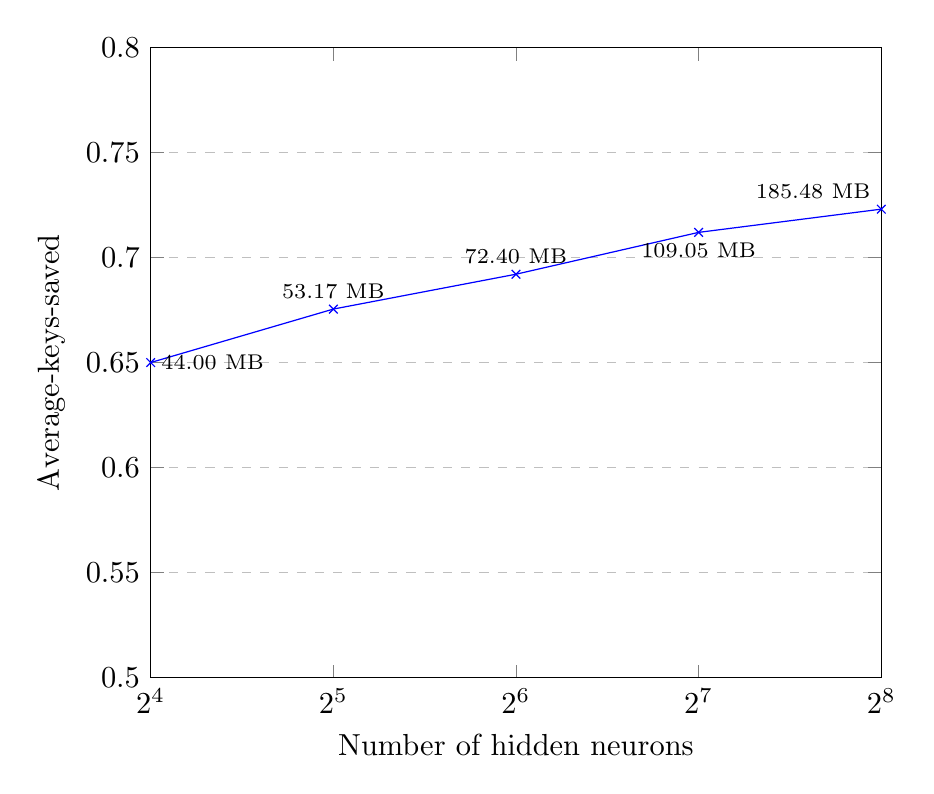
\begin{tikzpicture}[scale=1.1]
\begin{semilogxaxis}[
	scale only axis,
	xmin=16,xmax=256,
	log basis x=2,
	xtick={16, 32, 64, 128, 256},
	ymin=0.5,ymax=0.8,
	ymajorgrids=true,
	grid style=dashed,
	xlabel=Number of hidden neurons,
	ylabel=Average-keys-saved]

	\addplot[color=blue, mark=x]
	coordinates {(16, 0.65007)(32, 0.67552)(64, 0.69212)(128, 0.71204)(256, 0.72310)};
	\node [right] at (axis cs:  16, 0.65007) {\scriptsize 44.00 MB};
	\node [above] at (axis cs:  32, 0.67552) {\scriptsize 53.17 MB};
	\node [above] at (axis cs:  64, 0.69212) {\scriptsize 72.40 MB};
	\node [below] at (axis cs:  128, 0.71204) {\scriptsize 109.05 MB};
	\node [above left] at (axis cs:  256, 0.72310) {\scriptsize 185.48 MB};

\end{semilogxaxis}
\end{tikzpicture}
\caption{The effect of the number of hidden neurons on average-keys-saved and memory usage in a 2-layer vanilla RNN trained on the PTB dataset.}
\label{fig:average_keys_saved_vs_number_of_hidden_neurons}
\end{figure}

From figure~\ref{fig:average_keys_saved_vs_number_of_hidden_neurons}, it can be seen that much greater reductions in memory usage can be achieved for a given loss in average-keys-saved by decreasing the number of hidden neurons. Dropping from 256 to 32 hidden neurons in each layer gives a memory saving of 132.31 MB, with an average-keys-saved loss of 0.04758. It is intriguing that a 2-layer vanilla RNN with only 32 hidden neurons in each layer can achieve a better average-keys-saved score than the 5-gram model with Katz smoothing from figure~\ref{fig:ptb}. \\

Of course, there are several other techniques that can be used to optimise the memory and CPU overhead of language models for mobile platforms. These include, but are not limited to: reducing the number of hidden layers; using 16-bit floats for model parameters; removing the softmax layer from the RNN, since it is not strictly needed in ranking predictions; and memory-mapping the model to reduce memory pressure when it is initially being loaded.

\subsection{On Error-Prone Text} \label{error_prone_evaluation}

In this section I present my findings for the performance of language models on error-prone text. The goal is to produce a language model whose predictions are not deterred by errors in the input text, as illustrated in figure~\ref{fig:error_prone_to_error_free_rnn}. \\

Normally, language models are evaluated by feeding them a sequence of input words (the \tit{inputs}) and seeing how well they predict that same sequence of input words shifted forward in time by one word (the \tit{targets}). When evaluating my error-correcting language models, I did exactly the same thing, except that the inputs were allowed to contain errors in them and the targets were not. \\

\begin{figure}[h]
\captionsetup{justification=centering}
\centering
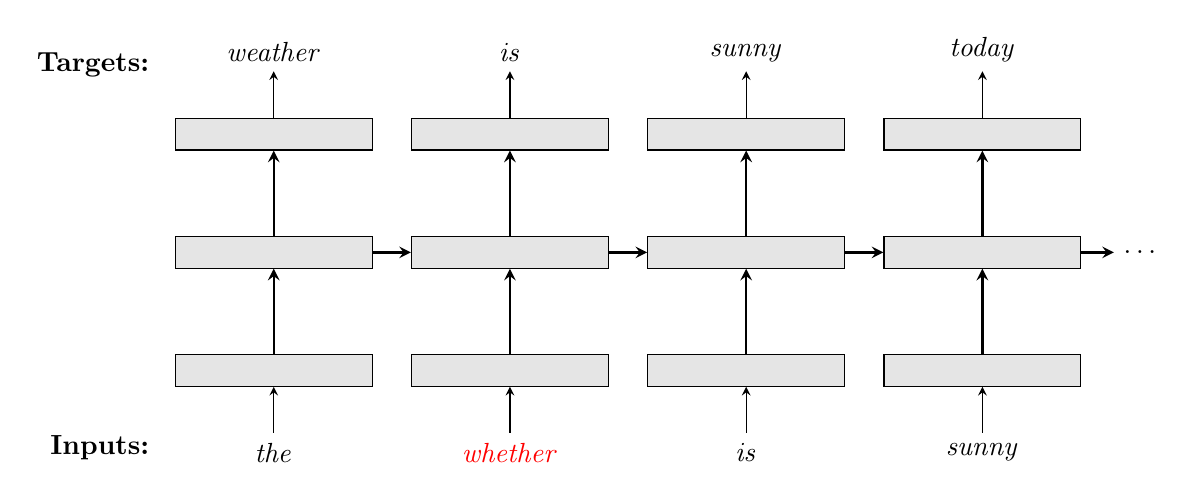
\begin{tikzpicture}[
		>=stealth,
		layer/.style={draw, rectangle, minimum width=25mm, minimum height=4mm, fill=black!10},
	]
	\node[layer] (input1) at (0, 0) {};
	\node[layer] (hidden1) at (0, 1.5) {};
	\node[layer] (output1) at (0, 3) {};
	\draw [<-] (input1) -- ++(0, -0.8) node [below] {\tit{the}};
	\draw [->, line width=0.3mm] (input1) -- (hidden1);
	\draw [->, line width=0.3mm] (hidden1) -- (output1);
	\draw [->] (output1) -- ++(0, 0.8) node [above] {\tit{weather}};
	
	\node[below left=5mm and 2mm of input1] (inputs) {\tbf{Inputs:}};
	\node[above left=4mm and 2mm of output1] (targets) {\tbf{Targets:}};

	\node[layer] (input2) at (3, 0) {};
	\node[layer] (hidden2) at (3, 1.5) {};
	\node[layer] (output2) at (3, 3) {};
	\draw [<-] (input2) -- ++(0, -0.8) node [below] {\textcolor{red}{\tit{whether}}};
	\draw [->, line width=0.3mm] (input2) -- (hidden2);
	\draw [->, line width=0.3mm] (hidden2) -- (output2);
	\draw [->] (output2) -- ++(0, 0.8) node [above] {\tit{is}};

	\node[layer] (input3) at (6, 0) {};
	\node[layer] (hidden3) at (6, 1.5) {};
	\node[layer] (output3) at (6, 3) {};
	\draw [<-] (input3) -- ++(0, -0.8) node [below] {\tit{is}};
	\draw [->, line width=0.3mm] (input3) -- (hidden3);
	\draw [->, line width=0.3mm] (hidden3) -- (output3);
	\draw [->] (output3) -- ++(0, 0.8) node [above] {\tit{sunny}};
	
	\node[layer] (input4) at (9, 0) {};
	\node[layer] (hidden4) at (9, 1.5) {};
	\node[layer] (output4) at (9, 3) {};
	\draw [<-] (input4) -- ++(0, -0.8) node [below] {\tit{sunny}};
	\draw [->, line width=0.3mm] (input4) -- (hidden4);
	\draw [->, line width=0.3mm] (hidden4) -- (output4);
	\draw [->] (output4) -- ++(0, 0.8) node [above] {\tit{today}};

	\node (cont) at (11, 1.5) {$\hdots$};

	\draw [->, line width=0.3mm] (hidden1.east) -- (hidden2.west);
	\draw [->, line width=0.3mm] (hidden2.east) -- (hidden3.west);
	\draw [->, line width=0.3mm] (hidden3.east) -- (hidden4.west);
	\draw [->, line width=0.3mm] (hidden4.east) -- (cont.west);
\end{tikzpicture}
\caption{The ideal error-correcting language model.}
\label{fig:error_prone_to_error_free_rnn}
\end{figure}

I used the CLC dataset, which consisted of six files:
\begin{center}
\begin{tabular}{c c}
	\ttt{train.correct.txt} & \ttt{train.incorrect.txt} \\
	\ttt{valid.correct.txt} & \ttt{valid.incorrect.txt} \\
	\ttt{test.correct.txt} & \ttt{test.incorrect.txt}
\end{tabular}
\end{center}
The training, validation and test sets all consisted of one file containing uncorrected text and another file containing the corresponding corrected text. I trained an 2-layer LSTM-based language model with 256 hidden neurons on \ttt{train.correct.txt}, and used \ttt{valid.correct.txt} to guide the learning rate decay. In order to focus the evaluation on the error-correcting ability of my language models, I removed any pairs of lines from the test set files that were identical. I also removed any pairs of lines that contained corrections that involve the insertion or deletion of words, because my model was not designed to handle these types of errors, as explained in section~\ref{error_correcting_lm}. \\

The ideal error-correcting language model would predict words as if the input were not error-prone, therefore, to obtain an \tit{upper bound} in performance, I evaluated the LSTM-based language model using \ttt{test.correct.txt} for the input words and \ttt{test.correct.txt} for the target words. In order to establish a \tit{lower bound}, I evaluated the performance of the same model using \ttt{test.incorrect.txt} for the input words and \ttt{test.correct.txt} for the target words. This model did not contain any error-correcting capabilities. \\

\begin{figure}[h]
\captionsetup{justification=centering}
\begin{adjustbox}{center}
\begin{tabular}{| L{6cm} | C{3cm} | C{5cm} |}
	\hline
	\tbf{Language model} & \tbf{Perplexity} & \tbf{Average-keys-saved} \\ \hline
	\tit{Upper bound} & 77.83 & 0.65483 \\ \hline
	\tit{Error-correcting LSTM}; $\delta$ = 1 & 87.99 & 0.64453 \\ \hline
	\tit{Error-correcting LSTM}; $\delta$ = 2 & 88.47 & 0.64376 \\ \hline
	\tit{Error-correcting LSTM}; $\delta$ = 3 & 88.57 & 0.64273 \\ \hline
	\tit{Lower bound} & 89.70 & 0.63912 \\ \hline
\end{tabular}
\end{adjustbox}
\caption{The performance of my error-correcting language model with respect to the upper and lower bound, using the CLC dataset.}
\label{fig:error_correcting_results}
\end{figure}

It can be seen from figure~\ref{fig:error_correcting_results} that my error-correcting model improves the performance of language model predictions on text containing errors that do not require the insertion or deletion of words. The best result arises from an edit distance threshold of 1, which seems attributed to the fact that a larger threshold allows for more false corrections, as shown in figure~\ref{fig:error_correcting_false}.

\begin{figure}[h]
\captionsetup{justification=centering}
\centering
\begin{subfigure}{\linewidth}
	\centering
	\begin{adjustbox}{center}
	\begin{tabular}{L{2.5cm} | L{12cm}}
		\tbf{Input} & i am more than happy to give you the \tbf{nessessary} information. \\ \hline
		\tbf{Target} & i am more than happy to give you the \tbf{necessary} information. \\ \hline
		\tbf{Prediction} & i am more than happy to give you the \tbf{necessary} information.
	\end{tabular}
	\end{adjustbox}
	\caption{An accurate correction.}
	\label{fig:error_correcting_good}
\end{subfigure}
~\\~\\
\begin{subfigure}{\linewidth}
	\centering
	\begin{adjustbox}{center}
	\begin{tabular}{L{2.5cm} | L{12cm}}
		\tbf{Input} & the bus will pick you up right at your hotel \tbf{entery}. \\ \hline
		\tbf{Target} & the bus will pick you up right at your hotel \tbf{entrance}. \\ \hline
		\tbf{Prediction} & the bus will pick you up right at your hotel \tbf{every}.
	\end{tabular}
	\end{adjustbox}
	\caption{A false correction.}
	\label{fig:error_correcting_false}
\end{subfigure}
~\\~\\
\begin{subfigure}{\linewidth}
	\centering
	\begin{adjustbox}{center}
	\begin{tabular}{L{2.5cm} | L{12cm}}
		\tbf{Input} & \tbf{appart of} that, there is no recommendation as to what to wear. \\ \hline
		\tbf{Target} & \tbf{apart from} that, there is no recommendation as to what to wear. \\ \hline
		\tbf{Prediction} & \tbf{apart of} that, there is no recommendation as to what to wear.
	\end{tabular}
	\end{adjustbox}
	\caption{A missed correction.}
	\label{fig:error_correcting_bad}
\end{subfigure}
\caption{Example corrections made by my error-correcting RNN with $\delta = 2$.}
\end{figure}

There is still a gap to be closed, which is demonstrated in figure~\ref{fig:error_correcting_bad} by the fact that my model does not correct non-spelling mistakes.

\chapter{Conclusions}

The project was a success: I implemented a variety of $n$-gram and RNN-based language models, and benchmarked them in terms of both their prediction performance and their applicability to running on a mobile platform, as set out in my project proposal. Additionally, I built a mobile keyboard for iOS that uses my language models as a library, and proposed a novel extension to an existing language model that improves its performance on error-prone text. \\

My implementation of existing language models saw a level of performance that was comparable with measures made by existing authors. For example, my 5-gram modified Kneser-Ney smoothing model, vanilla RNN model and LSTM model all matched the results from Mikolov on the Penn Tree Bank dataset~\cite{rnn_ptb:mikolov2012}~\cite{lstm_ptb:mikolov2014}. This allowed me to make comprehensive and reliable comparisons between each of my models, and assess the trade-offs between accuracy and resource consumption. My work also saw such models complement one another, in that the interpolation of their probability distributions surpassed the performance of all of my stand-alone models. \\

I explicitly demonstrated that language model performance is deterred by error-prone text. Whilst I made some modifications to an existing model that saw an increase in performance on such text, there is still room for improvement. If I were given more time to work on the project, I would investigate ways to cater for non-spelling corrections. From the CoNLL shared tasks of 2013~\cite{error_correction2013:ng2013} and 2014~\cite{error_correction2014:ng2014}, it is clear that there is a plethora of methods that already exist for grammatical error-correction. It would be interesting to see which of these could be applied to improve the performance of language models on error-prone text. \\

Throughout this dissertation, I have learnt a great deal about language modelling, but what have my language models learnt from me? Here is a one line summary of my work, in the words of an LSTM-based language model, trained on the significantly small training set that is the text of this \LaTeX\ file:

\begin{center}
\begin{tabular}{C{15cm}}
	\hline
	\tit{`the number of words that the language model is a mobile of the network, and the input is the input set.'} \\ \hline
\end{tabular}
\end{center}

% Get texcount to ignore the words in the bibliography, appendix and index.
%TC:ignore

%%%%%%%%%%%%%%%%%%%%%%%%%%%%%%%%%%%%%%%%%%%%%%%%%%%%%%%%%%%%%%%%%%%%%
% the bibliography
\newpage
\addcontentsline{toc}{chapter}{Bibliography}
\bibliographystyle{ieeetr}
\bibliography{bibliography}

%%%%%%%%%%%%%%%%%%%%%%%%%%%%%%%%%%%%%%%%%%%%%%%%%%%%%%%%%%%%%%%%%%%%%
% the appendices
\appendix

\chapter{Backpropagation Recurrence Relation} \label{appendix:bp_recurrence}

To see how the recurrence relation for $\delta_i^l$ is derived, consider the neuron $i$ in the first hidden layer of the neural network shown in figure~\ref{fig:backpropagation}. Without loss of generality, suppose this layer is layer $l$. \\

\begin{figure}[h]
\captionsetup{justification=centering}
\centering
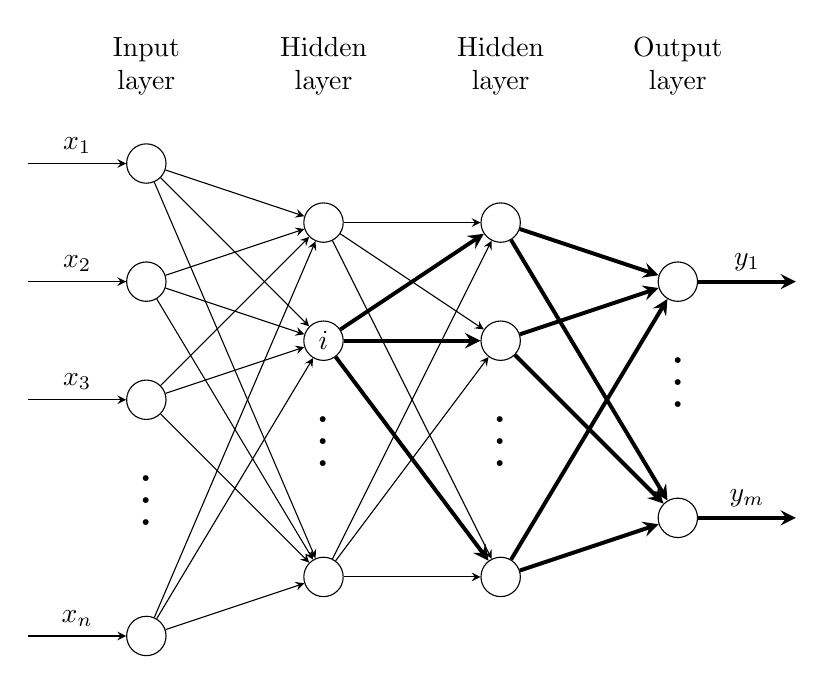
\begin{tikzpicture}[
	every neuron/.style={circle, draw, minimum size=5mm},
	neuron missing/.style={draw=none, scale=2, text height=0.1cm, execute at begin node=\color{black}$\vdots$},
	x=1.5cm,
	y=1.5cm,
	>=stealth
]

\foreach \m/\l [count=\y] in {1, 2, 3, missing, 4}
	\node [every neuron/.try, neuron \m/.try] (input-\m) at (0, 2.5-\y) {};

\foreach \m [count=\y] in {1, 2, missing, 3}
	\node [every neuron/.try, neuron \m/.try ] (hidden-\m) at (1.5, 2-\y) {};

\node (hidden-2-text) at (1.5, 0) {$i$};

\foreach \m [count=\y] in {1, 2, missing, 3}
	\node [every neuron/.try, neuron \m/.try ] (hidden-2-\m) at (3, 2-\y) {};

\foreach \m [count=\y] in {1, missing, 2}
	\node [every neuron/.try, neuron \m/.try ] (output-\m) at (4.5, 1.5-\y) {};

\foreach \l [count=\i] in {1, 2, 3, n}
	\draw [<-] (input-\i) -- ++(-1,0) node [above, midway] {$x_\l$};

\foreach \l [count=\i] in {1, m}
	\draw [->, line width=0.5mm] (output-\i) -- ++(1,0) node [above, midway] {$y_\l$};

\foreach \i in {1, ..., 4}
	\foreach \j in {1, ..., 3}
		\draw [->] (input-\i) -- (hidden-\j);

\foreach \i in {1, 3}
	\foreach \j in {1, ..., 3}
		\draw [->] (hidden-\i) -- (hidden-2-\j);

\foreach \j in {1, ..., 3}
	\draw [->, line width=0.5mm] (hidden-2) -- (hidden-2-\j);

\foreach \i in {1, ..., 3}
	\foreach \j in {1, ..., 2}
		\draw [->, line width=0.5mm] (hidden-2-\i) -- (output-\j);

\foreach \l [count=\x from 0] in {Input, Hidden, Hidden, Output}
	\node [align=center, above] at (\x*1.5, 2) {\l \\ layer};

\end{tikzpicture}
\caption{An illustration of the connections along which the partial derivatives are chained for backpropagating to a particular node $i$.}
\label{fig:backpropagation}
\end{figure}

From the diagram, it is clear that the derivative $\frac{\partial \mathcal{L}}{\partial z_i^l}$ depends on the derivatives of all of the neurons in layer $l + 1$, and so from the chain rule it follows that:
\begin{gather*}
	\frac{\partial \mathcal{L}}{\partial z_i^l} = \sum_j \frac{\partial \mathcal{L}}{\partial z_j^{l + 1}}\frac{\partial z_j^{l + 1}}{\partial z_i^l}
\end{gather*}
Plugging in the definition of $\delta_i^l$, and simplifying gives:
\begin{gather*}
	\delta_i^l = \sum_j \delta_j^{l+1} \frac{\partial z_j^{l+1}}{\partial z_i^l} = \sum_j \delta_j^{l+1} \frac{\partial z_j^{l+1}}{\partial y_i^l} \frac{\partial y_i^l}{\partial z_i^l} = \phi'(z_i^l) \sum_j \delta_j^{l+1} w_{i,j}^l
\end{gather*}
as required. \\

These ideas can be extended to a recurrent neural network, whereby the derivative $\frac{\partial \mathcal{L}}{\partial z_i^l}$ depends not only on the derivatives of the neurons in layer $l + 1$, but also on the neurons in layer $l$ at time step $t + 1$:
\begin{gather*}
	\frac{\partial \mathcal{L}}{\partial z_i^{l, t}} = \sum_j \frac{\partial \mathcal{L}}{\partial z_j^{l + 1, t}}\frac{\partial z_j^{l + 1, t}}{\partial z_i^{l, t}} + \sum_j \frac{\partial \mathcal{L}}{\partial z_j^{l, t + 1}}\frac{\partial z_j^{l, t + 1}}{\partial z_i^{l, t}}
\end{gather*}
Again, plugging in the definition of $\delta_i^{l, t}$ and simplifying gives:
\begin{gather*}
	\delta_i^{l, t} = \sum_j \delta_j^{l+1, t} \frac{\partial z_j^{l+1, t}}{\partial z_i^{l, t}} + \sum_j \delta_j^{l, t + 1} \frac{\partial z_j^{l, t + 1}}{\partial z_i^{l, t}} = \phi'(z_i^{l,t}) \big( \sum_j \delta_j^{l+1,t} w_{i,j}^l + \sum_j \delta_j^{l,t+1} v_{i,j}^l \big)
\end{gather*}
as required.

\chapter{Perplexity} \label{appendix:perplexity}

The formula for perplexity, presented in equation~\ref{eq:perplexity} and repeated below for convenience, can be better understood from a touch of information theory.
\begin{gather*}
	\text{PP}_L(w_1^N) = \sqrt[N]{\frac{1}{\mathbb{P}_L(w_1^N)}} = \sqrt[N]{\prod_{i=1}^{N}\frac{1}{\mathbb{P}_L(w_i | w_1^{i-1})}}
\end{gather*}
In information theory, the cross-entropy $H(p, q)$ between a true probability distribution $p$ and an estimate of that distribution $q$ is defined as:\footnote{Note that $H(p, q)$ is often also used to denote the joint entropy of $p$ and $q$, which is a different concept.}
\begin{gather*}
	H(p, q) = -\sum_x p(x) \log_2 q(x)
\end{gather*}
It can be shown that $H(p, q) = H(p) + D_{KL}(p || q)$ where $D_{KL}(p || q) \geq 0$ is the Kullback-Leibler distance between $p$ and $q$. Generally speaking, the better an estimate $q$ is of $p$, the lower $H(p, q)$ will be, with a lower bound of $H(p)$, the entropy of $p$. \\

The perplexity PP of a model $q$, with respect to the true distribution $p$ it is attempting to estimate, is defined as:
\begin{gather*}
	\text{PP} = 2^{H(p, q)}
\end{gather*}

Language models assign probability distributions over sequences of words, and so it seems reasonable to use perplexity as a measure of how accurately they model the real underlying distribution. Unfortunately, in language modelling, the underlying distribution, $p$, is not known, so it is approximated with Monte Carlo estimation by taking samples of $p$ (i.e. sequences of words from the test data) as follows:
\begin{gather*}
	\text{PP}_L(w_1^N) = 2^{-\frac{1}{N}\sum_i \log_2 \mathbb{P}_L(w_i | w_1^{i-1})}
\end{gather*}
With a little algebra, this can be rearranged to give equation~\ref{eq:perplexity}. \\

\chapter{Project Proposal}

%TC:endignore 

\end{document}


